\documentclass{article}
\usepackage{epigraph}
\usepackage{tikz}
\usepackage{graphicx}
\usepackage{float}
\usepackage[utf8]{inputenc}
\usepackage{pmboxdraw}
\usepackage{amsmath}
\usepackage{amsthm}
\usepackage{amsfonts}
\usepackage{amssymb}
\usepackage{bussproofs}
\usepackage{mathtools}
\usepackage{verbatim}
\usepackage{dsfont}
\usepackage{hyperref}
\usepackage{trfrac}
\usepackage{listings}
\usepackage{xcolor}
\usepackage{fancyvrb}

\definecolor{codegray}{rgb}{0.5,0.5,0.5}
\definecolor{backcolour}{rgb}{0.98,0.98,0.97}

\lstdefinestyle{mystyle}{
    backgroundcolor=\color{backcolour},
    commentstyle=\color{codegreen},
    numberstyle=\tiny\color{codegray},
    basicstyle=\ttfamily\footnotesize,
    breakatwhitespace=false,
    breaklines=true,
    captionpos=b,
    keepspaces=true,
    numbers=left,
    numbersep=5pt,
    showspaces=false,
    showstringspaces=false,
    showtabs=false,
    tabsize=2
}

\lstset{style=mystyle}

\hypersetup{colorlinks=true, linkcolor=black}

\theoremstyle{definition}
\newtheorem{definition}{Definition}

\theoremstyle{theorem}
\newtheorem{theorem}{Theorem}

\newcommand{\note}[1]{\textcolor{red}{\textit{#1}}}

\newcommand\level{\mathit{level}}
\newcommand\Ra{\Rightarrow}
\newcommand\ra{\rightarrow}
\newcommand\rab{\rightarrow_{\beta}}

\newcommand\dup{\mathrel{\mathtt{dup}}}
\newcommand\code{\mathtt}

\newcommand\SV{\SaveVerb}
\newcommand\UV{\UseVerb}

\newcommand\size{\mathit{size}}
\newcommand\uses{\mathit{uses}}
\newcommand\atlev{ \mathit{atLevel}}

\newcommand\fstsc{ \mathit{SC}_1}

\newcommand \sndsc{ \mathit{SC}_2}

\newcommand \thdsc{ \mathit{SC}_3} 
\newcommand \liff{ \longleftrightarrow}

\pagenumbering{arabic}

\begin{document}

\title{Moonad: A Peer-to-Peer Operating System}
\author{
  Victor Maia\\
  \texttt{victor.maia@ethereum.org}
  \and
  John Burnham\\
  \texttt{john.burnham@tezos.com}
}
\date{November 2019}
\maketitle

\setlength\epigraphwidth{.9\textwidth}
\setlength\epigraphrule{0pt}

\epigraph{\itshape But why, some say, the Moon? Why choose this as our goal? And
they may well ask, why climb the highest mountain? Why, 35 years ago, fly the
Atlantic? Why does Rice play Texas?}{---John F. Kennedy, \textit{Address at
Rice University on the Nation's Space Effort}}

\begin{abstract}
We present \textbf{Moonad}, a peer-to-peer operating system. Its machine
language, \textbf{FM-Net}, consists of a massively parallel, beta-optimal
graph-reduction system based on interaction nets. Its purely functional
user-facing language, \textbf{Formality} features a powerful, elegant
type-system capable of stating and proving theorems about its own programs
through inductive $\lambda$-encodings.  Online interactions are made through
\textbf{Bitlog}, a
token-less data-only blockchain, compatible with both private and decentralized
backends and featuring extensible smart contract universes. We
present two examples of such universes: \textbf{Ethos}, a universe with native
eWASM execution, and \textbf{Phos}, a universe with native FM-Net execution.

On top of those, we describe a front-end interface, Moonad, where users
can create, deploy and use decentralized applications in an immutable namespace,
transact in a trustless code and proof marketplace, and exchange digital assets.
\end{abstract}

\newpage
\tableofcontents
\newpage

\section{Introduction} 

Computing is a field in its infancy. While humans have performed manual
computation with fingers, pencil, abacus or quipu since time immemorial, it has
been only 75 years since the first general-purpose computing machine was
switched on. Given how ubiquitous computers are in our lives today, it can be
easy to forget this, but there are hundreds of millions still living who are
older than the computer. If a generation in human terms is 25 years, computers
users today are at most third-generation.

Accordingly, it should not be surprising that computing systems we use in
practice ---devices, operating systems, programming languages--- lag behind
(sometimes far behind) theoretical or experimental systems. Consider that the
most popular operating system in the world, Android was designed in the late
2000s, based on a kernel from the 1990s (Linux), which itself was based on a
design from the 1970s. There simply hasn't been enough time for all the good
ideas to be discovered and to percolate into common use.

For example, most electronic authentication on the web is still done with
passwords (sometimes stored in plain-text!), despite the fact that this
contributes to tens of billions of dollars lost per year to identity theft and
that secure systems for authentication based on public key cryptography have
existed for at least the past 30 years.

In a related area, most electronic commerce is mediated by centralized trusted
counterparties, despite the fact that this regularly leads to data breaches that
compromise the security of millions of people. Decentralized systems, such
cryptographic ledgers using byzantine-fault-tolerant chains of signed
transactions and trustless distributed computing platforms have been under
intense development for the better part of the past decade, but have yet to gain
widespread adoption.

There has been tremendous theoretical progress in programming language and
compiler design, that is barely exploited. We have substructural type systems
that can eliminate resource management errors (like segmentation faults) and
ensure memory safety. We have proof languages capable of unifying the field of
mathematics and programming as one (the Curry-Howard correspondence). In
principle, we could have systems software that is formally proven to be
error-free, and proof assistants that are both user-friendly enough to be taught
in grade-school math class and performant enough to be used on any platform.

Contrast this theoretical progress with our practical record: not long ago, we
had a single, small malicious package cause the entire web ecosystem to
collapse, twice. More than 300,000 sites online today are vulnerable to SQL
injections. Bugs like Heartbleed and TheDAO cause enormous monetary losses. A
single CPU exploit has slowed down nearly every processor in the world by 30%.
Faulty software kills people, routinely causing airplanes to crash and hospitals
to stop operating.

We believe this mismatch between theory and practice is due to presentation: The
technology exists, we need to build the user experience. Moonad aims to assemble
many of these amazing technologies into a decentralized operating system that
"just works"; to build computing systems that are fast, friendly and safe.

\section{Formality: An efficient programming proof language}

\subsection{Why a proof language?}

A proof language is as a programming language with a type system that is
sufficiently expressive to state and prove mathematical theorems about its own
programs. The Curry-Howard correspondence states that there is a structural
congruence between computer programs and proofs in formal logic. While in theory
this implies that software developers and mathematicians are engaged in
substantially the same activity, in practice there are many barriers preventing
the unification of the two fields. Programming languages with type systems
expressive enough to take advantage of Curry-Howard, such as Haskell, Agda and
Coq generally have substantial runtime overhead, which makes them challenging to
use, particularly at the systems programming level. On the other hand, systems
languages such as Rust, Nim or ATS, have shown that type systems can greatly
enhance usability and correctness of low-level software, but either have type
systems too weak to fully exploit Curry-Howard (Rust, Nim), or introduce
syntactic complexity that limits adoption (ATS). In other words, there are lots
of slow languages with great type systems and lots of fast languages with lousy
type systems.

As programmers and as mathematicians, we don't want to compromise. On one side,
mathematicians have the power of rigor: there is nothing more undeniably correct
than a mathematical proof. Yet ironically, those proofs are often written,
checked and reviewed by humans in an extremelly error-prone process. On the
other side, programmers have the power of automation: there is nothing more
capable of performing a huge set of tasks without making a single mistake than a
computer program. Yet, equally ironically, most of those programs are written in
an unrigorous, bug-ridden fashion. Formality lies in the intersection between
both fields: it is a programming language in which developers are capable of
implementing everyday algorithms and data structures, but it is also a proof
language, on which mathematicians are capable of proposing and proving theorems.

Types can be seen as a language of specfications that can be mechanically
checked by the compiler, allowing you to enforce arbitrary guarantees on your
program's behavior. For example, in an untyped language, you could write an
algorithm such as:

\begin{lstlisting}
// Returns the element at index `idx` of an array `arr`
function get_at(i, arr) {
  ... code here ...
}
\end{lstlisting}

But this has no guarantees. You could call it with nonsensical arguments such as
\verb|get_at("foo", 42)|, and the compiler would do nothing to stop you, leading
to (possibly catastrophical) runtime errors. Traditional typed languages improve
the situation, allowing you to "enrich" that definition with simple or even
polymorphic types, such as:

\begin{lstlisting}
function get_at<A>(i : Num, arr : Array<A>) : A {
  ... code here ...
}
\end{lstlisting}

This has some guarantees. For example, it is impossible to call \verb|get_at|
with a \verb|String| index, preventing a wide class of runtime errors. But you
can still, for example, call \verb|get_at| with an index out of bounds. In fact,
a similar error caused the catastrophic Heartbleed vulnerability. Formality
types are arbitrarily expressive, allowing you to capture all demands you'd
expect from \verb|get_at|:

\begin{lstlisting}
get_at*L : {A: Type, i: Fin(L), arr: Vector(A, L)} -> [x: A ~ At(A,L,i,arr,x)]
  ... implementation here...
\end{lstlisting}

Here, we use a bound, \verb|L|, to enforce that the index is not larger than the
size of the array, and we also demand that the returned element, \verb|x: A|, is
exactly the one at index \verb|i|. This specification is complete, in the
mathematical sense. It is not only impossible to get a runtime error by calling
\verb|get_at|, but it is also impossible to write \verb|get_at| incorrectly to
begin with.  Note that this is different from, for example, asserts or bound
checking.  Here, the compiler statically reasons about the flow or your program,
assuring that it can't go wrong with zero runtime costs.

In a similar fashion, you could use types to ensure that the balance of a
smart-contract never violates certain invariants, or that an airplane controller
won't push its nose down to a crashing position. Of course, you don't need to
write types so precise. If your software doesn't demand security, you could go
all way down to having fully untyped programs. The point is that the ability of
expressing properties so precisely is immensely valuable, specially when
developing critical software that demands all the security one can afford.

Some readers might object here that while formal proofs can ensure that a
program's implementation matches its specification, it cannot eliminate errors
inherent to the specification. This is true, but, in many cases, specifications
are much smaller than implementations. For example,

\begin{lstlisting}
spec : Type
  [
    // Demands a List function such that
    sort : List(Word) -> List(Word),

    // It returns the same list in ascendinig order
    And(is_same(xs, sort(ys)), is_ascending(sort(ys)))
  ]
\end{lstlisting}

The spec above demands a List function such that it returns the same list in
ascending order. Writing and auditing this specification is considerably easier
than implementing a complete sort function. As such, formal verification can be
seen as an optimization of human auditing: instead of verifying a vast amount of
code, you audit a small specification and let the compiler do the rest.

\subsection{Overview of Formality}

Formality is a new proof language designed to achieve 3 main goals:

\begin{enumerate}
\item Efficiency: it should be as fast as possible.
\item Simplicity: it should be implemented in as few lines of code as possible.
\item Accessibility: it should be usable by non-experts as much as possible.
\end{enumerate}

Existing proof languages such as Agda, Coq, Lean, Isabelle and Idris don't
address those goals with sufficient priority. They are often very slow, have big
implementations, and demand expert knowledge from its users. Formality achieves
efficiency by compiling to an efficient high-order machine featuring optimal
beta-reduction, no garbage-collection and massive parallelism. It achieves
simplicity by using as few core primitives as possible: in fact, every algorithm
and data-structure can be represented with just lambdas, including inductive
datatypes. It achieves accessibility by developing a syntax that is familiar to
regular developers, drawing insipration from popular languages like Python, Rust
and TypeScript.

Formality is a dependently typed programming language based on extrinsic type
theory. It is based on elementary terms are just annotated versions of the
Elementary Affine Lambda-Calculus (EALC), which is itself a terminating subset
of the lambda-calculus with great computational characteristics. In particular,
EALC is compatible with the most efficient version of the optimal reduction
algorithm [citation]. This is important because, while asymptically optimal,
most implementations of the algorithm carry an extra, significant constant
overhead caused by a book-keeping machinery. This made them too slow in
practice, decreasing interest on the area. By relying on EALC, we can avoid the
book-keeping overhead, making it much faster than all alternatives. Below is a
table comparing the amount of native operations (graph rewrites) required to
reduce $\lambda$-terms in other implementations and Formality:

 \begin{tabular}{ c | c | c | c | c | c}
Term & GeomOpt & GeomImpl & YALE & IntComb & Formality \\\hline
 22II &     204 &       56 &   38 &      66 &        21\\
222II &     789 &      304 &  127 &     278 &        50\\
  3II &      75 &       17 &   17 &      32 &         9\\
 33II &     649 &      332 &   87 &     322 &        49\\
322II &    7055 &     4457 &  383 &    3268 &        85\\
223II &    1750 &     1046 &  213 &     869 &        69\\
 44II &    3456 &     2816 &  148 &    2447 &        89\\
\end{tabular}

TODO: citations

Not only Formality requires orders of magnitude less native operations, but its
native operations are much simpler.

Unlike most proof languages, Formality doesn't include a datatype system, since
not only it is very complex to implement, which goes against our second goal
(simplicity), but can also cause more serious issues. For example, it was
discovered that type preservation does not hold in Coq due to its treatment of
coinductive datatypes [citation], and both Coq and Agda were found to be
incompatible with Homotopy Type Theory due to the K-axiom, used by native
pattern-matching on dependent datatypes [citation]. Instead, Formality relies on
lambda encodings, an alternative to a datatype system that use plain lambdas to
encode arbitrary data. While attractive, this approach wasn't adopted in
practical type theories for several reasons:


\begin{enumerate}
\item There is no encoding that provides both recursion and fast pattern-matching.
\begin{enumerate}
\item Church encodings provide recursion, but pattern-matching is slow $O(n)$.
\item Scott encodings provide fast pattern-matching, but no recursion.
\item Alternative encodings that provide both consume too much memory.
\end{enumerate}
\item We cannot prove \verb|0 != 1| with the usual definition of \verb|!=|.
\item Induction is not derivable.
\end{enumerate}

Formality solves the first issue by simply using Church encodings for recursion
and Scott encodings for data, the second issue by collapsing universes, and the
last issue by combining self-types and type-level recursion [citation]. It is
well-known that, in most proof languages, collapsing universes and type-level
recursion can lead to logical paradoxes, but the remarkable coincidence is that
the same feature that allows the language to be compatible with optimal
reductions, Elementary Affine Logic, also makes its type-theory sound in the
presence of those [proof]. This allows the theory to be remarkably simple and
powerful.

\subsection{EALC: Elementary Affine Lambda Calculus}
The Elementary Affine Lambda Calculus is a subset of the
$\lambda$-calculus which is both terminating and compatible with the
book-keeping free optimal reduction algorithm computed by FM-Net. Its terms are
defined by the following syntax:
\begin{definition} EALC terms

\SV{variable}|v|
\SV{lambdaTerm}|v => M|
\SV{lambdaApp}|M(N)|
\SV{boxedTerm}|#M|
\SV{boxedDup}|dup n = M; N|

Let $\mathbb{V}$ be an infinite set of variables $\{v_0,v_1,...,v_n\}$.
Let $\mathtt{v} \in \mathbb{V}$.

Then the EALC terms $\code{M,N}$ are defined recursively as:

\begin{align*}
\mathtt{M,N} &\Coloneqq \UV{variable} \tag*{(variable)}\\
  &\,\vert\, \UV{lambdaTerm}\tag*{(lambda term)}\\
  &\,\vert\, \UV{lambdaApp}\tag*{(lambda application)}\\
  &\,\vert\, \UV{boxedTerm}\tag*{(boxed term)}\\
  &\,\vert\, \UV{boxedDup}\tag*{(boxed duplication)}\\
\end{align*}
\end{definition}

The first 3 constructors are the usual $\lambda$-calculus. The last two
introduce boxes, which just wrap terms, and duplications, which copies the
contents of a box.

\subsubsection{EALC reduction}

Substitution of a variable in an EALC term is defined:
\begin{definition} EAlC substitution
  \begin{enumerate}
    \item \verb|x[y <- M]| is
      \begin{enumerate}
        \item if $\code{v} = \code{x}$ then $\code{M}$
        \item if $\code{v} \neq \code{x}$ then $\code{v}$
      \end{enumerate}
    \item \verb|(x => M)[y <- N]| is \verb|(x => M[y <- N])|
    \item \verb|(M(N))[x <- P]| is \verb|(M [x <-P])(N [x <- P])|
    \item \verb|(#M)[x <- N]| is \verb|#(M[x <- N])|
    \item \verb|(dup x = M; N)[y <- P]| is
          \verb|(dup x = M[x <- P]; N[y <- P])|
  \end{enumerate}
\end{definition}

The EALC has the following reduction rules:

\begin{definition} Single-step EALC reduction $\rab$

Let $[N/x]M$ indicate the substitution of $x$ by $N$ in $M$.

\SV{r1}|((x) => a)(b)|
\SV{r2}|a[x <- b]|
\SV{r3}|dup x = #a; b|
\SV{r4}|b[a <- x]|
\SV{r5}|((dup x = a; b) c)|
\SV{r6}|(b c)|
\SV{r7}|dup x = (dup y = a; b); c|
\SV{r8}|dup y = a; dup x = b; c|
\begin{enumerate}
\item application: $\UV{r1} \rab \UV{r2}$
\item duplication: $\UV{r3} \rab \UV{r4}$
\item appdup-swap: $\UV{r5} \rab \UV{r6}$
\item dupdup-swap: $\UV{r7} \rab \UV{r8}$
\end{enumerate}
\end{definition}

The first rule is the usual beta-reduction. The second rule allows us to copy
the contents of a box. The last two are just permutations, allowing inner $dup$s
to be exposed. A EALC term is said to be stratified when it follows the
following conditions:

\begin{definition} EALC stratification condition
\begin{enumerate}
\item Lambda-bound variables can only be used at most once.
\item There must be exactly 0 boxes between a variable bound by a lambda and its
   occurrence.
\item There must be exactly 1 box between a variable bound by a duplication and its
   occurrence.
\end{enumerate}
\end{definition}

The first condition says that lambdas must be affine. The second condition says
that lambdas can't substitute inside boxes. The third condition says that you
can't unbox, or add boxes, to a term by duplicating it. Stratified $\Lambda_!$
terms are strongly normalizing. 

Proof: TODO

\subsection{Formality Type Theory}

Formality Type Theory (FM-TT) extends the EALC with type annotations.

\subsubsection{Syntax}
FM-TT's syntax is defined as follows:

\begin{definition} FM-TT terms

\SV{variable}|v|
\SV{universe}|Type|
\SV{lambdaType}|(v : M) -> N|
\SV{lambdaTerm}|(v : M) => N|
\SV{lambdaApp}|M(N)|
\SV{boxedType}|!M|
\SV{boxedTerm}|#M|
\SV{boxedDup}|dup n = M; N|
\SV{selfType}|$v M|
\SV{selfTerm}|new(M) N|
\SV{selfElim}|%M|

\begin{align*}
\mathtt{M,N} &\Coloneqq \UV{variable} \tag*{(variable)}\\
  &\,\vert\, \UV{universe}\tag*{(universe)}\\
  &\,\vert\, \UV{lambdaType}\tag*{(lambda type, dependent product)}\\
  &\,\vert\, \UV{lambdaTerm}\tag*{(lambda term)}\\
  &\,\vert\, \UV{lambdaApp}\tag*{(lambda application)}\\
  &\,\vert\, \UV{boxedType}\tag*{(boxed type)}\\
  &\,\vert\, \UV{boxedTerm}\tag*{(boxed term)}\\
  &\,\vert\, \UV{boxedDup}\tag*{(boxed duplication)}\\
  &\,\vert\, \UV{selfType}\tag*{(self type)}\\
  &\,\vert\, \UV{selfTerm}\tag*{(self term)}\\
  &\,\vert\, \UV{selfElim}\tag*{(self elimination)}\\
\end{align*}
\end{definition}

For simplicity, we extend our notation with the following syntax sugars:

\begin{definition} FM-TT syntax sugars
\begin{itemize}
\item \verb|(x0 : A0, x1 : A1, ...) => t| for \\
      \verb|(x0 : A0) => (x1 : A1) => ... => t|
\item \verb|f(x,y,z)| for \verb|f(x)(y)(z)|
\item When \verb|x| isn't used in \verb|B|, \verb|A -> B| for \verb|(x : A) -> B|
\item We will also sometimes omit types of lambda-bound arguments when they can
be inferred and write \verb|(x0) => t| instead of \verb|(x : A) => t|
\end{itemize}
\end{definition}

Substitution of a variable in an FM-TT term is defined:
\begin{definition} FM-TT substitution
  \begin{enumerate}
    \item \verb|x[y <- M]| is
      \begin{enumerate}
        \item if $\code{v} = \code{x}$ then $\code{M}$
        \item if $\code{v} \neq \code{x}$ then $\code{v}$
      \end{enumerate}
    \item \verb|Type[y <- M]| is \verb|Type|
    \item \verb|(x : M -> N)[y <- P]| is \verb|(x : M[y <- P] -> N[y <- P])|
    \item \verb|(x : M => N)[y <- P]| is \verb|(x : M[y <- P] => N[y <- P])|
    \item \verb|(M(N))[x <- P]| is \verb|(M [x <- P])(N [x <- P])|
    \item \verb|(!M)[x <- N]| is \verb|!(M[x <- N])|
    \item \verb|(#M)[x <- N]| is \verb|#(M[x <- N])|
    \item \verb|(dup x = M; N)[y <- P]| is
          \verb|(dup x = M[x <- P]; N[y <- P])|
    \item \verb|($v M)[x <- N]| is \verb|$v M[x <- N]|
    \item \verb|(new(M)N)[x <- P]| is \verb|new(M[x <- P])N[x <- P]|
    \item \verb|(%M)[x <- N]| is \verb|%(M[x <- N])|
  \end{enumerate}
\end{definition}

\subsubsection{Typing Rules}

FM-TT's typing rules are:

\begin{definition} $\Lambda_F$ typing rules

\SV{v1}|(x : T)|
\SV{v2}|x : T|
\[ \trfrac[\small(variable)]
  {\UV{v1} \in \Gamma}
  {\Gamma \vdash \UV{v2}}
\]

\SV{tt}|Type : Type|
\[ \trfrac[\small(type-in-type)]
  {\varnothing}
  {\Gamma \vdash \UV{tt}}
\]

\SV{lT1}|A : Type|
\SV{lT2}|x : A|
\SV{lT3}|B : Type|
\SV{lT4}|(x : A) -> B : Type|
\[ \trfrac[\small(lambda type)]
  {\Gamma \vdash \UV{lT1}\quad \Gamma,\UV{lT2}\vdash\UV{lT3}}
  {\Gamma \vdash \UV{lT4}} 
\]

\SV{lt1}|A : Type|
\SV{lt2}|x : A|
\SV{lt3}|t : B|
\SV{lt4}|(x : A) => t : (x : A) -> B |
\[ \trfrac[\small(lambda term)]
  {\Gamma \vdash \UV{lt1}\quad \Gamma,\UV{lt2}\vdash\UV{lt3}}
  {\Gamma \vdash \UV{lt4}} 
\]

\SV{la1}|f : (x : A) -> B|
\SV{la2}|a : A|
\SV{la3}|f(a) : B[x <- a] |
\[ \trfrac[\small(lambda application)]
  {\Gamma \vdash \UV{la1}\quad \Gamma\vdash\UV{lt2}}
  {\Gamma \vdash \UV{la3}}
\]

\SV{bT1}|A : Type|
\SV{bT2}|!A : Type|
\[ \trfrac[\small(boxed type)]
  {\Gamma \vdash \UV{bT1}}
  {\Gamma \vdash \UV{bT2}}
\]

\SV{bt1}|t : A|
\SV{bt2}|#t : !A|
\[ \trfrac[\small(boxed term)]
  {\Gamma \vdash \UV{bt1}}
  {\Gamma \vdash \UV{bt2}}
\]

\SV{bd1}|t : !A|
\SV{bd2}|x : A|
\SV{bd3}|u : B|
\SV{bd4}| dup x = t; u : B|
\[ \trfrac[\small(boxed duplication)]
  {\Gamma \vdash \UV{bd1}\quad \Gamma,\UV{bd2}\vdash\UV{bd3}}
  {\Gamma \vdash \UV{bd4}}
\]

\SV{sT1}|s : $x A|
\SV{sT2}|A : Type |
\SV{sT3}|$x A : Type|
\[ \trfrac[\small(self type)]
  {\Gamma,\UV{sT1}\vdash\UV{sT2}}
  {\Gamma \vdash \UV{sT3}}
\]

\SV{st1}|t : A[x <- t]|
\SV{st2}|$x A : Type|
\SV{st3}|new($x A) t : $x A|
\[ \trfrac[\small(self term)]
  {\Gamma \vdash \UV{st1}\quad \Gamma\vdash\UV{st2}}
  {\Gamma \vdash \UV{st3}}
\]

\SV{se1}|t : $x A|
\SV{se2}|t : A[x <- t]|
\[ \trfrac[\small(boxed term)]
  {\Gamma \vdash \UV{se1}}
  {\Gamma \vdash \UV{se2}}
\]

\end{definition}

\subsubsection{Induction}

Those primitives allow FM-TT to be a simple type-theory featuring inductive
datatypes.

\begin{theorem} Induction can be proven in FM-TT
\end{theorem}

\begin{proof} \verb|nat_ind| in:

\begin{lstlisting}
Nat : Type
  $ self
  ( P    : Nat -> Type
  , succ : (r : Nat, i : P(r)) -> P(succ(r))
  , zero : P(zero)
  ) -> P(self)

succ : (n : Nat) -> Nat
  new(Nat) (P, succ, zero) => succ(n, (%n)(P, succ, zero))

zero : Nat
  new(Nat) (P, succ, zero) => zero

nat_ind :
  ( n : Nat
  , P : Nat -> Type
  , s : (n : Nat, i : P(n)) -> P(succ(n))
  , z : P(zero)) -> P(n)
  (n) => %n
\end{lstlisting}
\end{proof}

This defines an inductive lambda encoded datatype, \verb|Nat| as it's own
induction scheme. Mutual recursion is needed because the induction scheme of any
datatype refers to its constructors, which then refer to the defined datatype.
Self types are used because the type returned by the induction scheme can refer
to the term being induced. Together, those two components allow us to define
inductive datatypes with only ordinary lambdas. To induce on \verb|n : Nat| you
don't require any additional proof, all you need to do is eliminate its
self-type with \verb|%n|.  Note that this \verb|Nat| is complicated by the fact
it is recursive (Church encoded). We could have a non-recursive (Scott encoded)
\verb|Nat| as:

\begin{lstlisting}
Nat Type
  $ self
  ( ~P   : Nat -> Type
  , succ : (n : Nat) -> P(succ(n))
  , zero : P(zero)
  ) -> P(self)

succ(n : Nat) -> Nat
  new(Nat) (~P, succ, zero) => succ(n)

zero Nat
  new(Nat) (~P, succ, zero) => zero

nat_ind(n : Nat
       , ~P : Nat -> Type
       , s : (n : Nat, i : P(n)
       ) -> P(succ(n)), z : P(zero)) -> P(n)
  (n) => %n
\end{lstlisting}

Which is simpler and has the benefit of having constant-time pattern-matching.

Even simpler types include \verb|Bool|, \verb|Unit| and \verb|Empty|:

\begin{lstlisting}
Bool Type
  $ self
  ( ~P    : Bool -> Type
  , true  : P(true)
  , false : P(false)
  ) -> P(self)

true Bool
  new(Bool) (~P, true, false) => true

false Bool
  new(Bool) (~P, true, false) => false

bool_induction(b : Bool, ~P : Bool -> Type, t : P(true), f : P(false)) -> P(b)
  (b) => (%b)

Unit Type
  $ self
  ( ~P    : Unit -> Type
  , unit  : P(unit)
  ) -> P(self)

unit Unit
  new(Unit) (~P, unit) => unit

unit_induction(b : Unit, ~P : Unit -> Type, u : P(unit)) -> P(u)
  (u) => (%u)

Empty Type
  $ self
  ( ~P : Empty -> Type
  ) -> P(self)

empty_induction(b : Empty, ~P : Empty -> Type) -> P(b)
  (e) => (%e)
\end{lstlisting}

Notice how \verb|bool_induction| is equivalent to the elimination
principle of the \verb|Bool| datatype in Coq or Agda, except that in Formality
this was obtained without needing a complex datatype system implemented as
a native language feature. Formality's type theory is capable of expressing any
inductive datatype seen on traditional proof languages. For example,
\verb|Vector| (a list with statistically known length) can also be encoded as
its dependent elimination:

\begin{lstlisting}
Vector(~A : Type, len : Nat) -> Type
  $self
  ( ~P    : (len : Nat) -> Vector(A, len) -> Type
  , vcons :
      (~len : Nat
      , x : A
      , xs : Vector(A, len)
      ) -> P(succ(len), vcons(~A, ~len, x, xs))
  , vnil  : P(zero, vnil(~A))
  ) -> P(len, self)

vcons(~A : Type
     , ~len : Nat
     , head : A
     , tail : Vector(A, len)
     ) -> Vector(A, succ(len))
  new(Vector(A, succ(len))) (~P, vcons, vnil) => vcons(~len, head, tail)

vnil(~A : Type) -> Vector(A, zero)
  new(Vector(A, zero)) (~P, vcons, vnil) => vnil
\end{lstlisting}

And an identity type for propositional equality is just the J axiom wrapped by a
self type:

\begin{lstlisting}
Id(A : Type, a : A, b : A) -> Type
  $self
  ( ~P   : (b : A, eq : Id(A, a, b)) -> Type
  , refl : P(a, refl(~A, ~a))
  ) -> P(b, self)

refl(~A : Type, ~a : A) -> Id(A, a, a)
  new(Id(A, a, a)) (~P, refl) => refl
\end{lstlisting}

Formality is also able to express datatypes that traditional proof languages
can't. For example, intervals, i.e., booleans that can only be eliminated if
both provided cases are equal, can be written as:

\begin{lstlisting}
Interval Type
  $self
  ( ~P : (i : Interval) -> Type
  , I0 : P(i0)
  , I1 : P(i1)
  , SG : I0 == I1
  ) -> P(self)

i0 Interval
  new(Interval) (~P, i0, i1, sg) => i0

i1 Interval
  new(Interval) (~P, i0, i1, sg) => i1
\end{lstlisting}

And we can easily prove troublesome theorems like $0 /neq 1$: 

\begin{lstlisting}
true_isnt_false(e : Id(Bool, true, false)) -> Empty
  (%e)(~{b, e.b} (%e.b)(~{b}Type, Unit, Empty), unit)
\end{lstlisting}

This much type-level power comes at a cost: If Formality was based on the
conventional lambda calculus, it wouldn't be sound. However, since it is based
on EALC, a terminating untyped language, its normalization is completely
independent from types, so it is impossible to derive paradoxes by exploiting
non-terminating computations. A good exercise is attempting to write $\lambda x.
(x x) \lambda x.(x x)$ on EALC, which is impossible. 

The tradeoff is that EALC is considerably less computationally powerful than the
lambda calculus, imposing severe restrictions on how terms can be duplicated.
However in practice, this limitation isn't as onerous as might be expected.
Formality is still capable of modeling any algorithm that can be implemented in
a Turing Complete language, to some finite bound. Since all physical computing
systems also model Turing Complete computation to a finite time or space bound,
this means that Formality has the same level of practical expressivity as
common languages like C, Javascript or Haskell. Unlike those languages,
programming in Formality involves a resource-usage discipline that can be
burdensom to new users. We expect to develop advanced compiler tools for
automatic inference of boxed terms and types to ease the language acquisition
process.

Formality is currently being implemented in Javascript and Agda, the latter will
contain the formalization of Formality's consistency argument.


\subsection{Formality Lang: Numeric primitives and syntax sugar}

Formality Lang adds a series of user-friendly syntax sugars on top of EALC and
FM-TT making it much more usable.  It includes syntaxes for
datatype definitions and pattern-matching, loops, recursion, branching and so
on.
Formality Lang also adds native pairs, numbers and numeric operations. That is
done for efficiency reasons: native pairs use 1/3 of the space of lambda encoded
pairs, and native numbers can be stored unboxed on interaction net nodes, using
orders of magnitude less space than lambda encoded numbers.

Lastly, Formality Lang allows you to mark type information for erasure before
runtime. This reduces overhead during execution.


\subsubsection{Type Erasure}

TODO: Explain erasure

\subsubsection{Let}

Formality includes `let` expressions, which allow you to give local names to
terms.

\begin{lstlisting}
main : Output
  let hello = "Hello, world!"
  print(hello)
\end{lstlisting}

\verb|let| expressions can be infinitely nested.

\begin{lstlisting}
main : Output
  let output =
    let hello = "Hello, world!"
    print(hello)
  output
\end{lstlisting}

\subsubsection{Words}

The type of a native number is \verb|Word|. Words are unsigned integers of 32
bits:

\begin{lstlisting}
main : Word
  1900
\end{lstlisting}

They can also be written in hexadecimal:

\begin{lstlisting}
main : Word
  0x76C
\end{lstlisting}

And in binary:

\begin{lstlisting}
main : Word
  0b11101101100
\end{lstlisting}

They include many built-in operations:

\begin{tabular}{ c | c | c}
name & syntax & javascrip equivalent \\\hline
addition & \verb|x + y| & \verb|(x + y) >>> 0|\\
subtraction & \verb|x - y| & \verb|(x - y) >>> 0|\\
multiplication & \verb|x * y| & \verb|(x * y) >>> 0|\\
division & \verb|x / y| & \verb|(x / y) >>> 0|\\
modulus & \verb|x % y| & \verb|(x % y) >>> 0|\\
exponentiation & \verb|x ^ y| & \verb|(x ** y) >>> 0|\\
bitwise-and & \verb|x .& y| & \verb|x & y|\\
bitwise-or & \verb|x .& y| & \verb|x & y|\\
bitwise-xor & \verb|x .^ y| & \verb|x ^ y|\\
bitwise-not & \verb|.!(y)| & \verb|~y|\\
bitwise-right-shift & \verb|x .>> y| & \verb|x >>> y|\\
bitwise-left-shift & \verb|x .<< y| & \verb|x << y|\\
greater-than & \verb|x .> y| & \verb|x > y ? 1 : 0|\\
less-than & \verb|x .< y| & \verb|x < y ? 1 : 0|\\
equals & \verb|x .= y| & \verb|x === y ? 1 : 0|\\
float-addition & \verb|x +f y| & \verb|x + y|\\
float-subtraction & \verb|x -f y| & \verb|x - y|\\
float-multiplication & \verb|x *f y| & \verb|x * y|\\
float-division & \verb|x /f y| & \verb|x / y|\\
float-modulus & \verb|x %f y| & \verb|x % y|\\
float-exponentiation & \verb|x ^f y| & \verb|x ** y|\\
uint-to-float & \verb|.f(y)| & -\\
float-to-uint & \verb|.u(y)| & -\\
\end{tabular}
\\
\hfill
\newline
There is no operator precedence: parenthesis are always placed on the right.
That means 3 * 10 + 1 is parsed as 3 * (10 + 1). If you want the multiplication
to occur first, you must be explicit:

\begin{lstlisting}
main : Word
  (3 * 10) + 1
\end{lstlisting}

\subsubsection{If-Then-Else}

\verb|if| allows branching with a \verb|Word| condition.

 \hfill \newline
\begin{tabular}{ c | c }
syntax & description \\\hline
\verb|if n: a else: b| & If \verb|n .= 0|, evaluates to \verb|b|, else, evaluates to \verb|a|
\end{tabular}
\\ \hfill \newline

Usage is straightforward:

\begin{lstlisting}
main : Output
  let age = 30

  if age .< 18:
    print("boring teenager")
  else:
    print("respect your elders!")
\end{lstlisting}

\subsubsection{Pairs}

Native pairs store two elements of possibly different types.

\begin{tabular}{ c | c }
syntax & description \\\hline
\verb|[x : A, B(x)]| & The type of a pair\\
\verb|[a, b]| & Creates a pair with elements \verb|a| and \verb|b|\\
\verb|fst(p) | & Extracts the first element of a pair\\
\verb|snd(p) | & Extracts the second element of a pair\\
\verb|get [a, b] = p ... | &Extracts both elements of a pair\\
\end{tabular}
\\
\hfill
\newline

Note that the type of a pair is \verb|[x : A, B(x)]|, because the type of the
second element can depend on the value of the first. When it doesn't, you can
write just \verb|[:A, B]| instead. Using pairs is straightforward. Examples:

\paragraph{Creating:}

\begin{lstlisting}
main : [:Word, Word]
  [1, 2]
\end{lstlisting}

\paragraph{Extracting the first element:}

\begin{lstlisting}
main : Word
  let pair = [1, 2]
  fst(pair)
\end{lstlisting}

\paragraph{Extracting both elements:}

\begin{lstlisting}
main : Word
  let pair  = [1, 2]
  get [a,b] = pair
  a + b
\end{lstlisting}

\paragraph{Nesting to the left:}

\begin{lstlisting}
import Base@0

main : [:[:Word, Word], String]
  [[1, 2], "Hello Word!"]
\end{lstlisting}

\paragraph{Nesting to the right:}

\begin{lstlisting}
main : Word
  let triple  = [1, 2, 3] // same as [1, [2, 3]]
  get [x,y,z] = triple
  x + y + z
\end{lstlisting}

\paragraph{Erased (first element):}

\begin{lstlisting}
main : [~: Word, Word]
  [~1, 2] // the number "1" is erased from runtime
\end{lstlisting}

\paragraph{Erased (second element):}

\begin{lstlisting}
main : [: Word ~ Word]
  [1 ~ 2] // the number "2" is erased from runtime
\end{lstlisting}

Notably, the second element of a pair can depend on the value of the first.

\begin{lstlisting}
main : [x : Word, (if x: Word else: Bool)]
  [0, true] // if you change 0 to 1, the second element must be a Word.
\end{lstlisting}


\subsubsection{Datatypes}

Formality includes a powerful datatype system. A new datatype can be defined
with the `T` syntax, which is similar to Haskell's `data`, and creates global
definitions for its type and constructors. 

\begin{lstlisting}
T Bool
| true
| false
\end{lstlisting}

The unsugared Formality Lang type \verb|Bool| is essentially identical to FM-TT,
changing only the parenthesis \verb|(x : A)| in lambda types and terms to
brackets:

\begin{lstlisting}
Bool : Type
  $self
  { ~P    : {x : Bool} -> Type
  , true  : P(true)
  , false : P(false)
  } -> P(self)

true : Bool
  new(~Bool){~P, true, false} true

false : Bool
  new(~Bool){~P, true, false} false

case_of : {b : Bool, ~P : {x : Bool} -> Type, t : P(true), f : P(false)} -> P(b)
  (%b)(~P, t, f)
\end{lstlisting}

Some other examples of Formality datatypes are:

\begin{itemize}
\item Natural Numbers
\begin{lstlisting}
T Nat
| succ(n : Nat)
| zero
\end{lstlisting}

\item The Unit type
\begin{lstlisting}
T Unit
| unit
\end{lstlisting}

\item The Empty type
\begin{lstlisting}
T Empty
\end{lstlisting}

\item Vector
\begin{lstlisting}
T Vector (A : Type) (len : Nat)
| vcons(~len : Nat, head : A, tail : Vector(A, len)) : Vector(A, succ(len))
| vnil                                               : Vector(A, zero)
\end{lstlisting}

\item Equality
\begin{lstlisting}
T Equal (A : Type, a : A) (b : A)
| eq_refl : Equal(A, a, a)
\end{lstlisting}

\item The Interval type:
\begin{lstlisting}
T Interval
| i0
| i1
| i0 == i1
\end{lstlisting}

\end{itemize}

\paragraph{Enumerations}

Enumerations can be defined and used as follows:

\begin{lstlisting}
T Suit
| clubs
| diamonds
| hearts
| spades
\end{lstlisting}

To pattern-match against a value of a datatype, you must use `case/T`.

\begin{lstlisting}
print_suit : {suit : Suit} -> Output
  case/Suit suit
  | clubs    => print("First rule: you do not talk about Fight Club.")
  | diamonds => print("Queen shines more than diamond.")
  | hearts   => print("You always had mine.")
  | spades   => print("The only card I need is the Ace of Spades! \m/")
  : Output
\end{lstlisting}

The program above creates a datatype, \verb|Suit|, with 4 possible values. In
Formality, we call those values \textbf{constructors}. It then pattern-matches a
suit and outputs a different sentence depending on it. Notice that the \verb|case|
expression requires you to annotate the returned type. This is called the
\textbf{motive}, and is very useful when theorem proving. You can omit it by
using a \verb|case| argument instead:

\begin{lstlisting}
print_suit : {case suit : Suit} -> Output
| clubs    => print("First rule: you do not talk about Fight Club.")
| diamonds => print("Queen shines more than diamond.")
| hearts   => print("You always had mine.")
| spades   => print("The only card I need is the Ace of Spades! \m/")
\end{lstlisting}

\verb|case| arguments are shorter and simpler than \verb|case| expressions
but are less flexible.

\paragraph{Constructor with fields}

Datatype constructors can have fields, allowing them to store values:

\begin{lstlisting}
T Person
| person {age : Word, name : String}

get_name : {p : Person} -> String
  case/Person p
  | person => p.name
  : String
\end{lstlisting}

As you can see, fields can be accessed inside \verb|case| expressions and
\verb|case| arguments. Notice that \verb|p.name| is not a field accessor, but
just a single variable: the \verb|.| is part of its name. When Formality doesn't
know the name of the matched value, you must must explicitly name it using the
\verb|as| keyword:

\begin{lstlisting}
main : {p : Person} -> Word
case/Person person(26, "John") as john
| person => john.age
: Word
\end{lstlisting}
\begin{lstlisting}

\paragraph{Moving resources to branches:}

Since Formality functions are affine, you can't use an argument more than once.
So, for example, the function below isn't allowed:

\begin{lstlisting}
main : {a : Bool, b : Bool} -> Bool
  case/Bool a
  | true  => b
  | false => not(b)
  : Bool
\end{lstlisting}

In this case in particular, you used \verb|b| in two different branches, so you
shouldn't need to copy it. You can fix it with the \verb|move| keyword:

\begin{lstlisting}
main : {a : Bool, b : Bool} -> Bool
  case/Bool a
  + move b : Bool
  | true  => b
  | false => not(b)
  : Bool
\end{lstlisting}

Under the hoods, this is desugared to an extra lambda on each branch:

\begin{lstlisting}
main : {a : Bool, b : Bool} -> Bool
  (case/Bool a
  | true  => {b} b
  | false => {b} not(b)
  : Bool -> Bool)(b)
\end{lstlisting}

When using \verb|case| arguments, \verb|move|s are added automatically:

\begin{lstlisting}
main : {case a : Bool, b : Bool} -> Bool
| true  => b
| false => not(b)
\end{lstlisting}

As you can see, the version using \verb|case| arguments is the shortest.

\paragraph{Dependent motives}

In Formality, the type returned by a case expression can depend on the matched
value. For example, we can do this:

\begin{lstlisting}
main : Word
  case/Bool true as x
  | true  => 42
  | false => "hello"
  : case/Bool x
    | true  => Word
    | false => String
    : Type
\end{lstlisting}

While strange-looking, this is prefectly logical and well-typed. The reason this
works is that, when checking the type of a \verb|case| expression, Formality
first specializes the motive for *every possible branch* to determine "what it
demands". In this case, it demands a \verb|Word| on the \verb|true| branch, and
a \verb|String| on the \verb|false| branch. If you satisfy every demand, then it
determines the type of the whole \verb|case| expression by specializing the
motive using actual matched value. In this case, we matched on \verb|true|, so
it returns \verb|Word|.

We could write a function that returns different types based on its input:

\begin{lstlisting}
foo : {case b : Bool} -> case/Bool b | true => Word | false => String : Type
| true  => 42
| false => "hello"

main : Word
  foo(true) + foo(true)
\end{lstlisting}

Note this is not the same as returning \verb|Either|, which is done in Haskell
when we want to return different types, needing an extra pattern-match every
time you call the function. Here, that's not necessary, because \verb|foo|
really returns different types based on its input. Thanks to dependent types,
Formality can statically determine if you're doing the right thing, so,
replacing \verb|foo(true)| by \verb|foo(false)| would be a type error

\paragraph{Functions with different return types}

We could write a function that returns different types based on its input:

\begin{lstlisting}

foo : {case b : Bool} -> case/Bool b \verb| true => Word \verb| false => String : Type
| true  => 42
| false => "hello"

main : Word
  foo(true) + foo(true)
\end{lstlisting}

Note this is not the same as returning \verb|Either|, which is done in Haskell when we want to return different types, needing an extra pattern-match every time you call the function. Here, that's not necessary, because \verb|foo| really returns different types based on its input. Thanks to dependent types, Formality can statically determine if you're doing the right thing, so, replacing \verb|foo(true)| by \verb|foo(false)| would be a type error.

paragraph{ Proving absurds with Empty}

Another interesting example comes from the \verb|Empty| datatype:

\begin{lstlisting}
T Empty
\end{lstlisting}

This code isn't incomplete, the datatype has zero constructors. This means it is
impossible to construct a term \verb|t| with type \verb|Empty|, but we can still
accept it as a function argument. So, what happens if we pattern match against
it?

\begin{lstlisting}

wtf : {x : Empty} -> ???
  case/Empty
  : ???
\end{lstlisting}

The answer is: we can replace \verb|???| by anything, and the program will
check. That's because we technically proved all the demanded cases, so Formality
just returns the motive directly as the type of this \verb|case| expression.
That allows us to write a function that returns something absurd:

\begin{lstlisting}

prove_1_is_2 : {e : Empty} -> 1 == 2
  case/Empty e
  : 1 == 2
\end{lstlisting}

If we managed to call it, we'd have a proof that \verb|1 == 2|, which is absurd,
making Formality inconsistent. But this is fine: \verb|prove_1_is_2| can't ever
be called, because we can't construct a value of type \verb|Empty|. This is
pretty useful, so we have a base-lib function that, given an element of
\verb|Empty|, returns any absurd type:

\begin{lstlisting}
absurd : {e : Empty, ~P : Type} -> P
  case/Empty e
  : P
\end{lstlisting}

The opposite holds too: given an absurd equality, we can make an element of type
\verb|Empty|. Here is an example:

\begin{lstlisting}

true_isnt_false : {e : true == false} -> Empty
  unit :: rewrite x
    in case/Bool x
       \verb| true  => Unit
       \verb| false => Empty
       : Type
    with e
\end{lstlisting}

As an exercise, convince yourself why this works.

paragraph{ Unreachable branches with equality notes}

Notice the program below:

\begin{lstlisting}
import Base@0

main : Word
  case/Bool true
  | true  => 10
  | false => ?
  : Word
\end{lstlisting}

Here, we're matching against \verb|true|, so we know the \verb|false| case is
unreachable, but we still need to fill it with something. In this case, we could
write any number, but that's not always possible. In those cases, equality notes
can be helpful:

\begin{lstlisting}
import Base@0

main : Word
  case/Bool true as x
  + note e : x is true
  \verb| true  => 10
  \verb| false => absurd(false_isnt_true(e), ~Word)
  : Word
\end{lstlisting}

The \verb|+ note e : x == true| syntax reminds Formality that \verb|x == true|,

making it specialize \verb|x| on each branch, giving you an
\verb|e : true == true| on the \verb|true| branch, and an 
\verb|e : false == true| on the \verb|false| branch. Since \verb|false == true|
is absurd, we know the \verb|false| branch is unreachable and, thus, can fill it
by exploiting the \verb|absurd| function above, without writing any number.

To desugar an equality note, Formality simply adds an extra, erased equality
argument:

\begin{lstlisting}
import Base@0

main
  (case/Bool true as x
  \verb| true  => {~e} 10
  \verb| false => {~e} absurd(false_isnt_true(e), ~Word)
  : {~e : x == true} -> Word)(~refl(~true))
\end{lstlisting}

Notice that the left side of the equality note is allowed to access the matched
value (\verb|x|), while the right side is used to build the \verb|refl| proof.

paragraph{ Recursive fields}

Fields can refer to the datatype being defined:

\begin{lstlisting}
// {- From Data.Nat -}
T Nat
| succ {pred : Nat}
| zero
\end{lstlisting}

Since \verb|Nat| is so common, there is a syntax-sugar for it: \verb|0n3|, which
expands to \verb|succ(succ(succ(zero)))|.

Mutual recursion is allowed:

\begin{lstlisting}
T Foo
| foo {bar : Foo}

T Bar
| bar {foo : Bar}
\end{lstlisting}

And negative occurrences too:

\begin{lstlisting}
T Loop
| loop {f : Foo -> Foo}
\end{lstlisting}

While recursion is very liberal on types, the same isn't true for programs. You
can't write recursive functions directly, such as:

\begin{lstlisting}
mul_by_2 : {case n : Nat} -> Nat
| succ => succ(succ(mul_by_2(n)))
| zero => zero

main : Nat
  mul_by_2(0n2)
\end{lstlisting}

This makes dealing with recursive datatypes more complex than usual, since you
must use a boxed definition:

\begin{lstlisting}
#mul_by_2*N : !{case n : Nat} -> Nat
| succ => succ(succ(mul_by_2(n)))
| zero => zero
halt: zero

#main : !Nat
  <mul_by_2*>(0n2)
\end{lstlisting}

paragraph{ Polymorphism }

Polymorphic datatypes allow us to create multiple instances of the same datatype
with different contained types.

\begin{lstlisting}
import Base@0

T Pair {A : Type, B : Type}
| pair {x : A, y : B}

main : Word
  let a = pair(~Bool, ~Word, true, 7)

  case/Pair a
  \verb| pair => a.y
  : Word
\end{lstlisting}

The \verb|{A : Type, B : Type}| after the datatype declares two polymorphic
variables, \verb|A| and \verb|B|, allowing us to create different types of pair,
such as a pair of Bool, or a pair of Word, without needing to duplicate the
definition of \verb|Pair|. Each polymorphic variable adds an implicit, erased
argument to each constructor, so, instead of \verb|pair(true, 7)|, you need to
write \verb|pair(~Bool, ~Word, true, 7)|. In a future, this verbosity will be
prevented with implicit arguments. For now, you can amend it with a \verb|let|:

\begin{lstlisting}
import Base@0

T Pair {A : Type, B : Type}
| pair {x : A, y : B}

main : [:Pair(Bool, Bool), Pair(Bool, Bool)]
  let pairbb = pair(~Bool, ~Bool)

  let a = pairbb(true, false)
  let b = pairbb(false, true)
  [a, b]
\end{lstlisting}

By combining polymorphism with recursive types, we can create the popular
\verb|List| type (already defined on the base libs above):

\begin{lstlisting}
// T List {T : Type}
// \verb| cons {head : T, tail : List(T)}
// \verb| nil

// Returns all but the first element
// tail : {~T : Type, case list : List(T)} -> List(T)
// \verb| cons => list.tail
// \verb| nil  => nil(~T)

main : List(Word)
  tail(~Word, cons(~Word, 1, cons(~Word, 2, cons(~Word, 3, nil(~Word)))))
\end{lstlisting}

Since \verb|List| is so common, there is a built-in syntax-sugar for it, the
dollar sign:

\begin{lstlisting}
main : List(Word)
  tail(~Word, Word$[1, 2, 3])
\end{lstlisting}

paragraph{Indices}

Indices are like polymorphic variables, except that, rather than constant types,
they are \emph{computed values} that can depend on each constructor's arguments.
That gives us a lot of type-level power, and is one of the reasons Formality is
a great proof language. For example:

\begin{lstlisting}
T IsEven (x : Word)
| make_even {half : Word} (half * 2)
\end{lstlisting}

This datatype has one index, \verb|x|, of type \verb|Word|. Its constructor,
\verb|is_even|, has one field, \verb|half : Word|. When you write
\verb|make_even(3)|, the number \verb|3| is multiplied by two and moved to the
type-level, resulting in a value of type \verb|IsEven(6)|. So, for example:

\begin{lstlisting}
even_0 : IsEven(0)
  make_even(0)

even_2 : IsEven(2)
  make_even(1)

even_4 : IsEven(4)
  make_even(2)

even_6 : IsEven(6)
  make_even(3)
\end{lstlisting}

Notice that is is \emph{impossible} to create a value with type
\verb|IsEven(3)|, because that would require a \verb|half : Word| such that
\verb|half * 2 == 3|, and there is no such number. Because of that, indexed
datatypes have many applications. For example, suppose that you want to write a
\verb|div2| function that divides a number by two, but you don't want it to be
called with odd numbers. You could do this:

\begin{lstlisting}
div2 : {x : Word, ~x_is_even : IsEven(x)} -> Word
  x / 2

main : Word
  div2(10, ~make_even(5))
\end{lstlisting}

Here, the second argument "proves" that the first is even, making it impossible
to call \verb|div2| with an odd input. Since \verb|x_is_even| is erased from the
runtime, this gives us a static, zero-cost guarantee. Alternatively, we could
have used \verb|~x_is_even : [k : Word ~ x == k * 2]|, but indexed datatypes are
more handy in general. For example, you could easily write one for 3 consecutive
numbers:

\begin{lstlisting}
T Consecutive (a : Word, b : Word, c : Word)
| consecutive {init : Word} (init, init + 1, init + 2)
\end{lstlisting}

So, for example, \verb|Consecutive(a, b, c)| means \verb|a|, \verb|b|, \verb|c|
are 3 consecutive numbers such as \verb|7, 8, 9|. You could also write a type
for sorted lists:

\begin{lstlisting}
T SortedList {A : Type} (xs : List(Word))
| scons {
  add  : Word,
  head : Word,
  tail : List(Word),
  prof : SortedList(Word, cons(~Word, head, tail))
} (cons(~Word, head + add, cons(~Word, head, tail)))
| snil
   (nil(~Word))
\end{lstlisting}

Here, \verb|SortedList(xs)| would mean that \verb|xs| is a list of \verb|Word|s
with elements in descending order, such as \verb|[7, 5, 5, 3, 1]|. In order
words, a function that returned \verb|[xs : List(Word) ~ SortedList(xs)]| could
only be written if \verb|xs| was, indeed, sorted. And so on. Indexed datatypes,
in a way, give us a powerful language of specifications which we can use to
statically reason about our datatypes and algorithms.

For a more complex example of indices, here is a Vector, which is like a
\verb|List|, except that its type stores its own length:

\begin{lstlisting}hakell
 T Vector {A : Type} (len : Nat)
 | vcons {~len : Nat, head : A, tail : Vector(A, len)} (succ(len))
 | vnil                                                (zero)
\end{lstlisting}

Every time we call vcons, the len index on the type of the vector increases by one, allowing us to track its length statically:

\begin{lstlisting}
main : Vector(String, 0n3)
   vcons(~String, ~0n2, "ichi",
   vcons(~String, ~0n1, "ni",
   vcons(~String, ~0n0, "san",
   vnil(~String))))
\end{lstlisting}

This has many applications. For example, we can create a type-safe \verb|vhead|
that returns the first element of a non-empty vector:

\begin{lstlisting}
vhead : {~T : Type, ~n : Nat, xs : Vector(T, succ(n))} -> T
   case/Vector xs
   + note e : xs.len is succ(n)
   | vcons => xs.head
   | vnil  => absurd(zero_isnt_succ(~n, ~e), ~T) 
   : T
\end{lstlisting}

Notice that constructor indices are accessible on the left side of an equality
note. That gives us an \verb|e : zero == succ(n)| (since \verb|zero| is the
length of \verb|vnil|, and \verb|succ(n)| is the length of \verb|xs|). Since
\verb|0 != 1|, this branch is unreachable, so we can fill it with an
\verb|absurd|.

\subsubsection{Recursion}

TODO: explain recursion

\subsection{FM-Net: A massively parallel low-level machine language}

Formality terms are compiled to a memory-efficient interaction net system called
FM-Net. Interaction nets are graphs where nodes have labeled ports, one
being the main one, plus a list of "rewrite rules" that are activated whenever
two nodes are connected by their main ports. A simple interaction-net
graph-rewrite system called "interaction combinators" with only 3 symbols and 6
rules has been shown to be a universal model of computation. As a universal
model, interaction-nets combine many useful properties of other models such as
Turing machines and the lambda calculus. Like Turing machines, interactions-nets
can be evaluated as a series of atomic, local operations with a clear physical
implementation. Like the lambda calculus, interaction-nets are inherently
parallel, but in a more robust manner, admitting desirable computational
properties such as strong confluence, optimal sharing and zero-cost
garbage-collection.

Formality uses a slightly modified version of interaction combinators, called
FM-Net as our lowest-level machine language, extending interaction combinators
with additional graph node types for efficient numeric operations. This
implementation has advantages over previous interaction net graph-reduction
systems (such as the Bologna Optimal Higher-order Machine) in that it requires
no book-keeping, requires only 128 bits per lambda or pair, has unboxed 32-bit
integers and constant-time beta reduction. This is possible due to Formality's
stratification, a structural discipline on how terms are duplicated, inherited
from its underlying logic, Elementary Affine Lambda Calculus.

\subsubsection{Node Types}

\begin{figure}[H]
  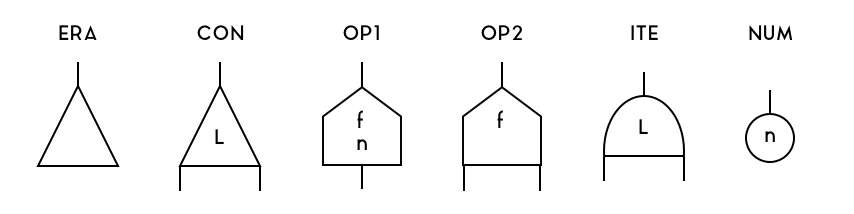
\includegraphics[width=\linewidth]{fm-net-node-types.png}
  \caption{FM-Net Node Types}
\end{figure}

Our FM-Net system includes 6 types of nodes, \verb|ERA|, \verb|CON|, \verb|OP1|,
\verb|OP2|, \verb|ITE|, \verb|NUM|.

\begin{enumerate}
\item \verb|CON| has 3 ports and an integer label. It is used to represent lambdas,
  applications, boxes (implicitly) and duplications. Just `CON` is enough for
  beta-reduction.

\item \verb|ERA| has 1 port and is used to free empty memory, which happens when a
  function that doesn't use its bound variable is applied to an argument.

\item \verb|NUM| has 1 port and stores an integer and is used to represent native
  numbers.

\item \verb|OP1| has 2 ports and stores one integer and an operation \verb|f|.
\verb|OP2| has 3 ports and an operation \verb|f|. They are used for numeric
operations such as addition and multiplication.

\item \verb|ITE| has 3 ports and an integer label. It is used for if-then-else,
and is required to enable number-based branching.  
\end{enumerate}

Note that the position of the port matters. The port on top is called the
\verb|main| port. The first port counter-clockwise to the main port (i.e., to
the left on this drawing) is the \verb|aux0| port, and the first port clockwise
to the main port (i.e., to the right on this drawing) is the \verb|aux1| port.

\subsubsection{Rewrite rules}

In order to perform computations, FM-Net has a set of rewrite rules that are
triggered whenever two nodes are connected by their main ports. This is an
extensive list of those rules:

\begin{figure}[H]
  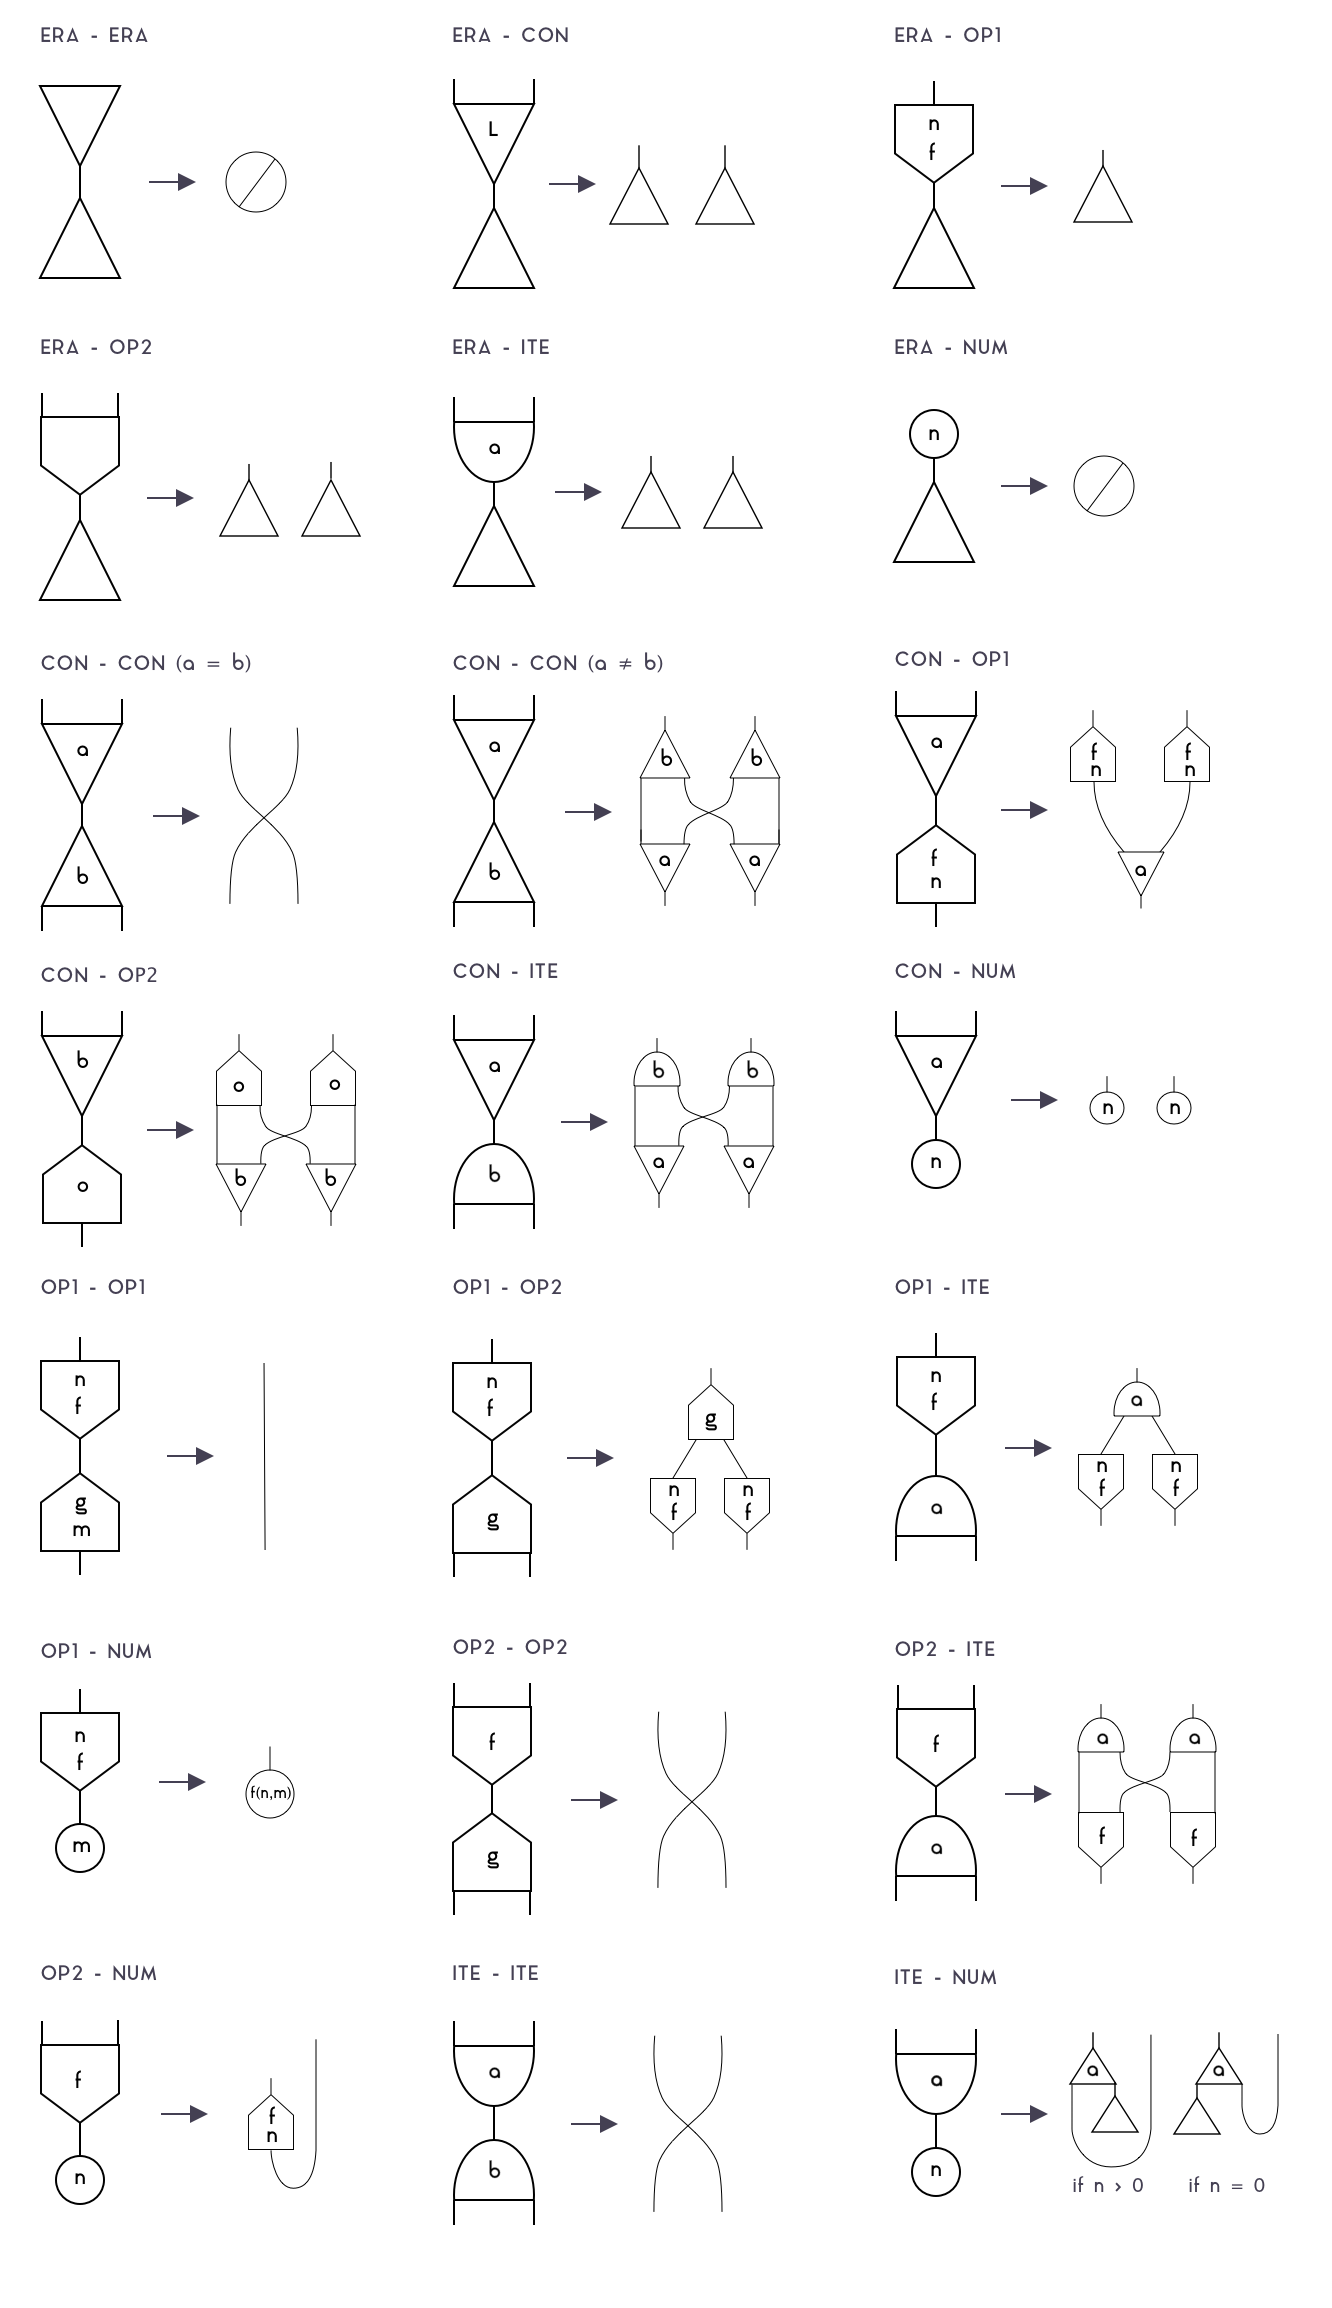
\includegraphics[width=\linewidth]{fm-net-rewrite-rules.png}
  \caption{FM-Net Node Types}
\end{figure}

Note that, while there are many rules (since we need to know what to do on each
combination of a node), most of those have the same "shape" (such as
\verb|OP2-OP2|, \verb|ITE-ITE|), so they can reuse the same code. There are only
5 actually relevant rules:

\begin{enumerate}
  \item \textbf{Erasure:} When an \verb|ERA| or a \verb|NUM| node collides with
  anything, it "destroys" the other node, and propagates itself to destroy all
  nodes connected to it.

  \item \textbf{Substitution:} When two \verb|CON| nodes of equal label collide,
  and also on the \verb|OP2-OP2| / \verb|ITE-ITE| cases, both nodes are
  destroyed, and their neighbors are connected.  That's the rule that performs
  beta-reduction because it allows connecting the body of a lambda (which is
  represented with \verb|CON|) to the argument of an application (which is, too,
  represented with \verb|CON|). Note that on the OP2-OP2 and ITE-ITE cases,
  that's just a default rule that doesn't matter, since those cases can't happen
  on valid FM-Core programs.

  \item \textbf{Duplication:} When different nodes collide, they "pass through"
  each other, duplicating themselves in the process. This allows, for example,
  \verb|CON| nodes with a label \verb|>1| to be used to perform deep copies of
  any term, with \verb|dup x = val; ...|. It can copy lambdas and applications
  because they are represented with \verb|CON| nodes with a label \verb|0|,
  pairs and pair-accessors, because they are represented with \verb|CON| nodes
  with a label \verb|1|, and \verb|ITE|, \verb|OP1|, \verb|OP2|, because they
  are different nodes.

  It also allows duplications to duplicate terms that are partially duplicated
  (i.e., which must duplicate, say, a $\lambda$-bound variable), as long as the
  \verb|CON| labels are different, otherwise, the \verb|CON| nodes would instead
  fall in the substitution case, destroying each other and connecting neighbors,
  which isn't correct. That's why FMC's box system is necessary: to prevent
  concurrent duplication processes to interfere with each other by ensuring
  that, whenever you duplicate a term with \verb|dup x = val; ...|, all the
  duplication \verb|CON| nodes of \verb|val| will have a labels higher than the
  one used by that \verb|dup|.

  \item \textbf{If-Then-Else:} When an \verb|ITE| node collides with a
  \verb|NUM| node, it becomes a \verb|CON| node with one of its ports connected
  to an \verb|ERA| node. That's because then/else branches are actually stored
  in a pair, and this allows you to select either the \verb|fst| or the
  \verb|snd| value of that pair and discard the other branch.

  \item \textbf{Num-Operation:} When \verb|OP2| collides with a \verb|NUM|, it
  becomes an \verb|OP1| node and stores the number inside it; i.e., the binary
  operation becomes a unary operation with \verb|NUM| partially applied. When
  that \verb|OP1| collides with another \verb|NUM|, then it performs the binary
  operation on both operands, and return a new \verb|NUM| with the result.
  Those rules allow us to add, multiply, divide and so on native numbers.
\end{enumerate}

\subsubsection{FM-Core Compiling to FM-Net}

The process of compiling FM-Core to FM-Net can be defined by the following
function \verb|k_b(net)|:

\begin{figure}[H]
  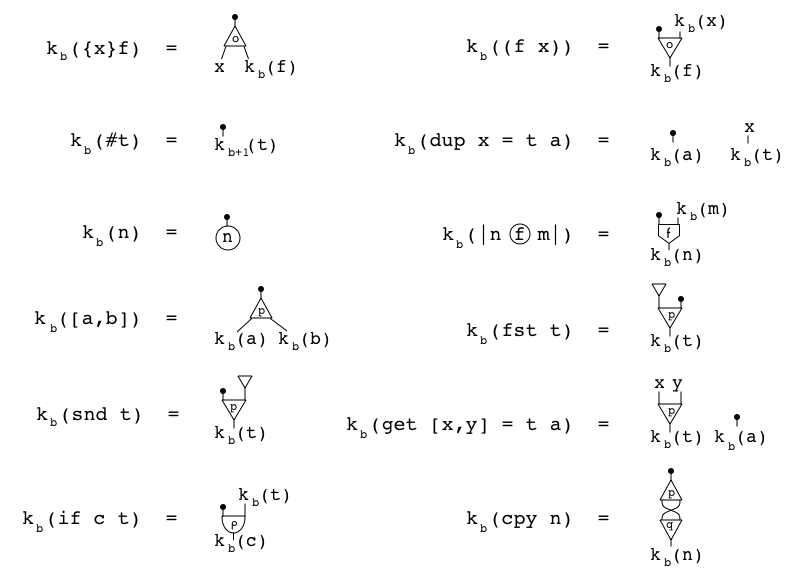
\includegraphics[width=\linewidth]{fm-net-compilation.png}
  \caption{FM-Net Node Types}
\end{figure}

This function recursively walks through a term, creating nodes and "temporary
variables" (\verb|x_b|) in the process. It also keeps track of the number of
boxes it passed through, \verb|b|. For example, on the lambda (\verb|{x}f|)
case, the procedure creates a \verb|CON| node with a label \verb|0|, creates a
"temporary variable" \verb|x_b| on the \verb|aux0| port, recurses towards the
body of the function, \verb|f| on the \verb|aux1| port, and then returns the
\verb|main| port (because there is a black ball on it).  Notice that there isn't
a case for \verb|VAR|. That's what those "temporary variables" are for. On the
\verb|VAR| case, two things can happen:

\begin{enumerate}
  \item If the corresponding "temporary variable" \verb|x_b| was never used,
  simply return a pointer to it.

  \item If the corresponding "temporary variable" \verb|x_b| was used, create a
  \verb|CON| node with a label \verb|2 + b|, connect its main port to the old
  location of \verb|x_b|, its \verb|aux0| to the port \verb|x_b| pointed to, and
  return a pointer to its \verb|aux1| port.
\end{enumerate}

This process allows us to create as many \verb|CON| nodes as needed to duplicate
\verb|dup|-bound variables, and labels those nodes with the layer of that
\verb|dup| (plus 2, since labels 0 and 1 are used for lambdas/applications and
pairs/projections). Note that this process is capable of duplicating
$\lambda$-bound variables, but this isn't safe in practice, and won't happen in
well-typed inputs.

\subsubsection{Implementation}

In our implementation, we use a buffer of 32-bit unsigned integers to represent
nodes, as follows:

\begin{enumerate}
  \item \verb|CON|: represented by 4 consecutive uints. The first 3 represent
  the \verb|main|, \verb|aux0| and \verb|aux1| ports. The last one represents
  the node type (2 bits), whether its ports are pointers or unboxed numbers (3
  bits), and the label (27 bits).

  \item \verb|OP1|: represented by 4 consecutive uints. The first 2 represent
  the \verb|main| and \verb|aux0| ports. The third represents the stored number.
  The last one represents the node type (2 bits), whether its ports are pointers
  or unboxed numbers (3 bits, 1 unused), and the operation (27 bits).

  \item \verb|OP2|: represented by 4 consecutive uints. The first 2 represent
  the \verb|main|, \verb|aux0| and \verb|aux1| ports. The third represents the
  stored number. The last one represents the node type (2 bits), whether its
  ports are pointers or unboxed numbers (3 bits), and the operation (27 bits).

  \item \verb|ITE|: represented by 4 consecutive uints. The first 2 represent
  the \verb|main|, \verb|aux0| and \verb|aux1| ports. The third represents the
  stored number. The last one represents the node type (2 bits), whether its
  ports are pointers or unboxed numbers (3 bits), and the label (27 bits).

  \item \verb|ERA|: is stored inside other nodes and do not use any extra space.
  An \verb|ERA| node is represented by a pointer port which points to itself.
  That's because \verb|ERA|'s rewrite rules coincide with what we'd get if we
  allowed ports to point to themselves.

  \item \verb|NUM|: is stored inside other nodes and do not use any extra space.
  A \verb|NUM| node is represented by a numeric port. In order to know if a port
  is a number or a pointer, each node reserves 3 bits of its last uint to store
  that information.
\end{enumerate}

\subsubsection{Rewrites}

TODO: explain how \verb|rewrite| works, how \verb|link_ports| is used, and why
\verb|unlink_ports| is necessary to avoid invalid states.

\subsubsection{Strict evaluation}

The strict evaluation algorithm is very simple. First, we must keep a set of
redexes, i.e., nodes connected by their main ports. In order to do that,
whenever we link two main ports, we must add the address of the smallest nodes
to that set. We then perform a loop to rewrite all redexes. This will give us a
new set of redexes, which must then be reduced again, over and over, until there
are no redexes left. This is the pseudocode:

\begin{lstlisting}[language=Python]
while (len(net.redexes) > 0):
  for redex in net.redexes:
    net.rewrite(redex)
\end{lstlisting}

The strict reduction is interesting because it doesn't require graph walking nor
garbage collection passes, and because the inner \verb|for|-loop can be
performed in parallel. That is, every \verb|redex| in \verb|net.redexes| can be
rewritten at the same time.

In order to do that, though, one must be cautious with intersection areas. For
example, in the graph below, B-C and D-E are redexes. If we reduce them in
parallel, both threads will attempt to read/write from C's and D's \verb|aux0|
and \verb|aux1| ports, potentially causing synchronization errors.

\begin{figure}[H]
  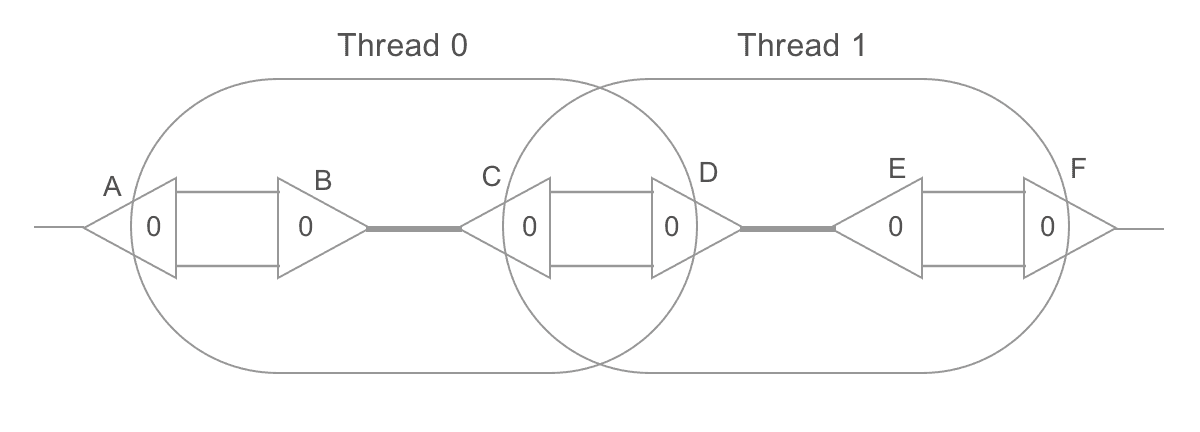
\includegraphics[width=\linewidth]{sk_problem_2x.png}
  \caption{Multithread reduction intersection}
\end{figure}

This can be avoided through locks, or by performing rewrites in two steps. On
the first step, each thread reads/writes the ports of its own active pair as
usual, except that, when it would need to connect a neighbor, it instead turns
its own node into a "redirector" which points to where the neighbor was supposed
to point. For example, substitution and duplication would be performed as
follows:

\begin{figure}[H]
  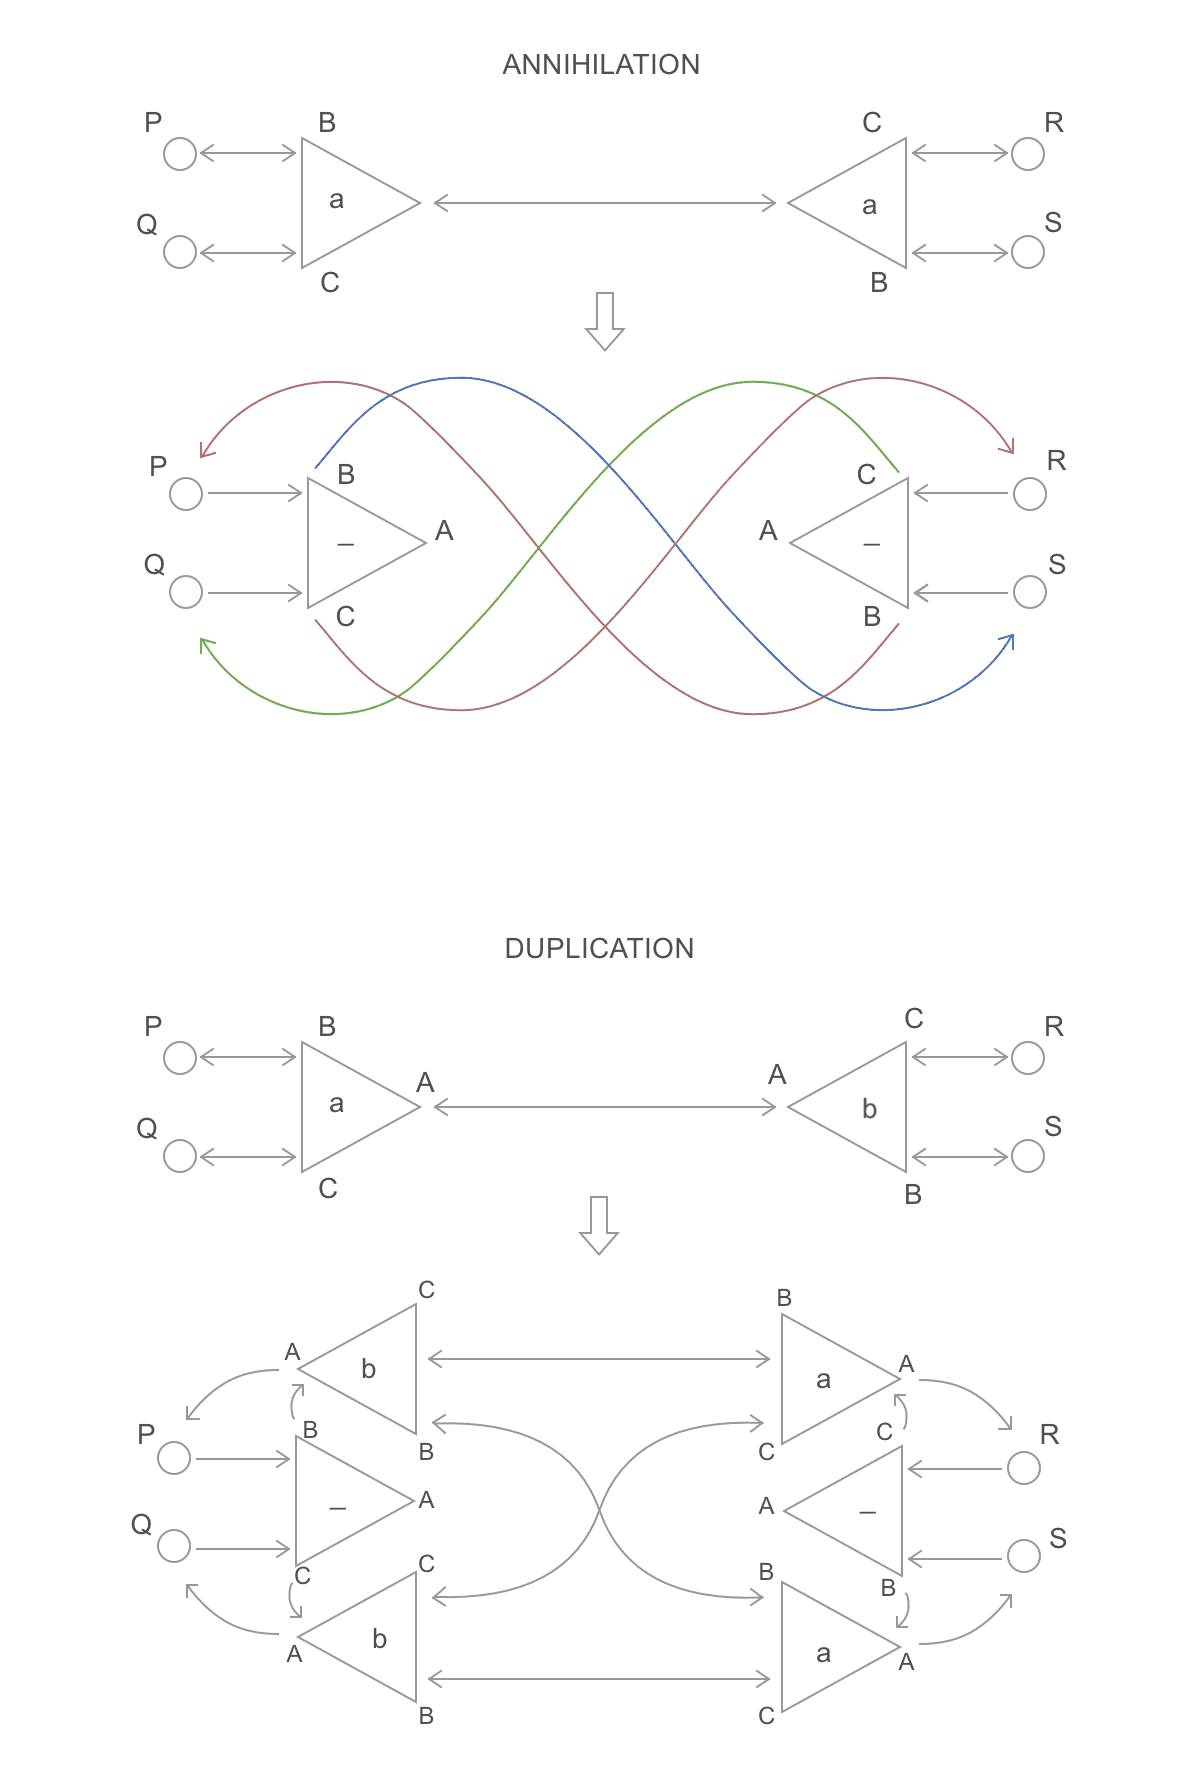
\includegraphics[width=\linewidth]{sk_local_rewrites_2x.png}
  \caption{Two step local rewrites}
\end{figure}

Notice that \verb|P|, \verb|Q|, \verb|R| and \verb|S| (neighbor ports) weren't
touched: they keep pointing to the same ports, but now those ports point to
where they should point to. Then, a second parallel step is performed. This
time, we spawn a thread for each neighbor port and walk through the graph until
we find a non-redirector node. We then point that neighbor to it. Here is a full
example:

\begin{figure}[H]
  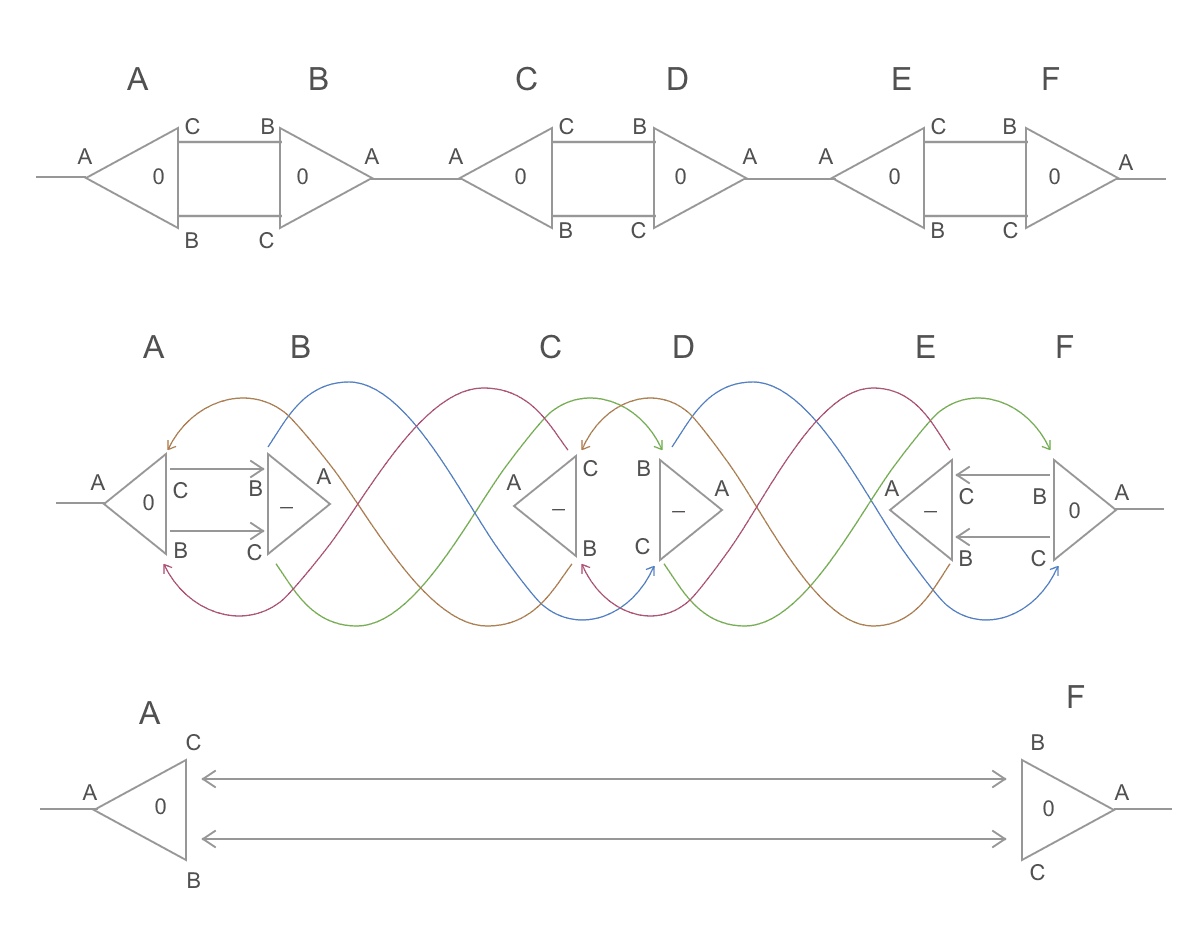
\includegraphics[width=\linewidth]{sk_local_rewrites_ex_2x.png}
  \caption{Example}
\end{figure}

Notice, for example, the port \verb|C| of the node \verb|A|. It is on the
neighborhoods of a redex (\verb|B-C|), but isn't a redex itself. On the first
step, two threads rewrite the nodes \verb|B-C| and \verb|D-E|, turning them into
redirectors, and without touching that port. On the second step, a thread starts
from port \verb|C| of node \verb|A|, towards port \verb|B| of node \verb|B| (a
redirector), towards port \verb|C| of node \verb|D| (a redirector), towards port
\verb|B| of node \verb| F|. Since that isn't a redirector, the thread will make
\verb|C| point to \verb|B|. The same is done for each neighbor port (in
parallel), completing the parallel reduction.

\subsubsection{Lazy evaluation}

The lazy evaluation algorithm is very different from the strict one. It works by
traversing the graph, exploring it to find redexes that are "visible" on the
normal form of the term, skipping unnecessary branches. It is interesting
because it allows avoiding wasting work; for example, \verb|({a b}b (F 42) 7)|
would quickly evaluate to \verb|7|, no matter how long \verb|(F 42)| takes to
compute. In exchange, it is "less parallel" than the strict algorithm (we can't
reduce all redexes since we don't know if they're necessary), and it requires
global garbage collection (since erasure nodes are ignored).

To skip unnecessary branches, we must walk through the graph from  port to port,
using a strategy very similar to the denotational semantics of symmetric
interaction combinators. First, we start walking from the root port to its
target port. Then, until we get back to the root, do as follows:

\begin{enumerate}
  \item If we're walking from an aux port towards an aux port of a node, add the
  aux we're coming from to a stack, and move towards the main port of that node.

  \item If we're walking from a main port to an auxiliary port, then we just
  found a node that is part of the normal form of the graph! If we're performing
  a weak-head normal form reduction, stop. Otherwise, start walking towards each
  auxiliary port (either recursively, or in parallel).

  \item If we're walking towards root, halt.
\end{enumerate}

This is a rough pseudocode:

\begin{lstlisting}[language=Python]
def reduce_lazy(net, start):
  back = []
  prev = start
  next = net.enter(prev)

  while not(net.is_root(next)):
    if slot_of(prev) == 0 and slot_of(next) == 0:
      net.rewrite(prev, next)
    elif slot_of(next) == 0:
      for aux_n from 0 til net.aux_ports_of(next):
        net.reduce_lazy(Pointer(node_of(next), aux_n))
    else:
      back.push(prev)
      prev = Pointer(node_of(next), 0)
      next = net.enter(prev)
\end{lstlisting}

While the lazy algorithm is inherently sequential, there is still an opportunity
to explore parallelism whenever we find a node that is part of the normal form
of the graph (i.e., case \verb|2|). In that case, we can spawn a thread to walk
towards each auxiliary port in parallel; i.e., the \verb|for|-loop of the
pseudocode can be executed in parallel like the one on the strict version. This
would allow the algorithm to have many threads walking through the graph at the
same time.  Again, caution must be taken to avoid conflicts.

\subsubsection{Performance}

TODO: comparative benchmarks and asymptotic behavior.

\subsubsection{FPGA}

TODO: describe our plans for FPGA compilation

\section{Bitlog: A token-less data-only blockchain}

\subsection{Overview}
Many current blockchain platforms rely on a built-in token to maintain
protocol incentives (block rewards) and to fund development via speculation (the
ICO model). This has often lead to incentives misalignment, poor platform
governance, securities fraud and corresponding regulatory overreaction.
However built-in tokens are not a necessary feature of blockchain platforms: A
modification of Proof of Work based Nakomoto Consensus can still function in the
absence of such a built-in token, while still preserving Byzantine Fault
Tolerance under certain assumptions. In essence, Proofs of Work themselves can
act as the scarce, though non-fungible, resource which secures the network.
Furthermore, a flexible data-only transaction format and extensible state
transition functions enable full application generality, including extrinsic
emulation of the the built-in tokens and incentives of other platforms. Full
cryptoeconomic abstraction can be achieved without loss of security or
scalability, enabling competition between different candidate block-reward
tokens and therefore market discovery of what computational characterisics are
desired by the platform at any given time.

\subsection{A brief history of blockchains}

In 2009, Bitcoin was created as a purely peer-to-peer electronic cash system.
While successful at achieving money-like characterstics (store-of-value,
medium-of-exchange) in a low-trust setting, Bitcoin is functionally limited due
to the constraint of being, essentially, just a map of balances with a limited
set of transactions.

Decentralized economic interactions often require complex rules to be enforced,
which Bitcoin often struggles to express at the protocol level. This limitation
resulted on the creation of a vast amount of application-specific decentralized
networks such as Namecoin, for name registering, or Monero, for built-in
privacy. This state-of-affairs is wasteful and inefficient, since competing
application-specific platforms can't easily interact or exchange value.

In 2013, Ethereum attempted to solve this constraint by generalizing Bitcoin
with an embedded Turing-complete scripting language. This allowed the protocol
to be arbitrarily extended by users through custom state-machines called
"smart-contracts". The vision was that Ethereum would eventually incorporate
most specific use-cases, allowing decentralized applications to coexist and
interact in the same network. Sadly, this has been inhibited by lack of
efficiency. Emulating computations like linked ring signatures or zk-snarks on
a virtual machine is prohibitely more expensive than application-specific
blockchains that can execute fast native implementations.

To solve Ethereum's scalability issues, alternative smart-contract blockchains
such as Tezos or Ethereum 2.0 propose moving from Proof-of-Work to 
Proof-of-Stake based consensus. If Proof of Work is conceptualized as
probabalistic voting proportional to computing power, Proof-of-Stake is a
probabalistic vote based on ownership of a built-in token. In effect,
Proof-of-Stake internalizes the capital embodied in the Proof-of-Work miners'
computing hardware. While Proof-of-Stake is theorized to be more scalable than
Proof-of-Work, practical implementation has faced many challenges
(nothing-at-stake, platform centralization, weak subjectivity, securities
regulation, etc.), requiring increased protocol complexity.

Increased protocol compleity in turn implies a larger space of potential
platforms, each with its own set of trade-offs and chosen parameters. Not only
does this increase cross-platform friction, on an individual blockchain every
new built-in feature developed makes that platform less efficient for the set of
users that don't need or care about that feature. For example, if a user is
only interested in publishing proofs of existence, then everything else is
wasteful: signatures, accounting, virtual machines. Yet, when they make a
transaction on Bitcoin or Ethereum, they are indirectly subsidizing all those
things. The more features a blockchain has, the less efficient it becomes for
any given user.

\subsection{Bitlog: Less is more}

Bitlog has the same design goal as Ethereum, implementing a decentralized
smart-contract platform, but takes the opposite approach: Instead of extending
Bitcoin with a bunch of new features and a fully-featured virtual machine,
Bitlog removes almost all existing features to the point there is only the
blockchain left. That is, Bitlog removes the "coin" from Bitcoin, leaving us
with only the bits: a token-less, data-only chain of blocks.

Blockchain platforms are fundamentally interpretation functions on top of a
stream of ordered events. A platform's consensus mechanism ensures that
participants in a network arrive at agreement on that event-stream.
A platform's protocol is function that allows the computation of a global state
from that event-stream: \verb| Event -> WorldState -> WorldState|

However, nothing prevents subsets of participants from running a second
interpretation, or state-transition, function on the same event-stream as the
first. In Bitcoin, for instance the \verb|OP_RETURN| opcode allows for the
creation of what are called "Null Data" transactions: Transactions which do
nothing other than embed arbitrary bits (up to 83 bytes) into the blockchain.
While these "Null Data" transactions are ignored by the Bitcoin protocol, it is
feasible to construct an alternate intrepretation function that discards all
\emph{other} transactions except those that are Null Data and e.g. whose bytes
contain some digital signature.

Consider the Namecoin blockchain for example. Instead of making a whole new
blockchain, Namecoin's users could just agree on a transition function, say,
\verb|namecoin(tx, state)|, which, given an array of transactions, would compute
the state of the network.  They could then embbed their namecoin transactions as
Null Data transactions on Bitcoin, using it as a stream of events. As long as
users are happy to pay Bitcoin fees, Namecoin can live "on top" of
Bitcoin.

Bitlog is a generalization of this idea of "Null Data" embedding. It is a
blockchain that contains, effectively, only "Null Data" transactions, and 
then supports a variety of custom transition functions built upon that event
stream.

\subsection{Why Bitlog will grow}

Bitlog is extremely future-proof. Cryptocurrencies and smart-contract platform
are destined to become obsolete because developers continually find better ways
to implement the same features. Ethereum, for example, has a huge set of
sub-optimal opcodes that will be changed on its next version. The problem is
that protocol changes require forks, which split a blockchain in two and
threaten consensus. If Ethereum was, instead, an interpretation function on top
of Bitlog, then, changing the protocol would only require users to agree on a
new "interpretation function". If they disagree, there would still be a fork,
but it would be a logical one, since both interpretation functions would still
read from the same stream of events. Equally, after some time had passed after a
logical fork, a new interpretation function could reintegrate the two differing
subjective "universes" back into a single worldstate. That is, on Bitlog there
is not only forking, but also the inverse operation of merging.

Since Bitlog doesn't have any bloat, it is arguably the least expensive way to
publish ordered, decentralized events. Since that is the essence of
decentralized applications, people are incentived to create platforms as
interpretation functions on top of Bitlog. If a platform decides to fork, then
its users will download different interpretation functions, but, since Bitlog is
the least expensive way to publish transactions, they're incentived to still use
the same blockchain. In other words, Bitlog forks don't fork the blockchain,
making it a snowball that only gets bigger. The only reason to fork the
blockchain would be if one found a cheaper way to publish transactions, which,
in a PoW setting, is impossible, because you can't optimize something that does
nothing.

\subsection{Implementation and incentives}

In implementation Bitlog really isn't that innovative: it is, literally, just
Bitcoin without the coin, for a small but significant efficiency gain. 

It consists of a chain of blocks, where each block cointains a set of
transactions / events, which are just blobs of bits, i.e., they contain no
structure, signature, amounts, inputs nor outputs. Every 1 minute, a block is
mined by proof-of-work. The miner includes as many transactions as possible on
the block header by taking the merkle root of the transaction set. The
difficulty is adjusted every Y blocks.  There will be a block size limit, but
possibly much larger than what Bitcoin is currently capable of. And so on. This
raises one obvious questions: if there is no coin, what incentives miners have
to keep mining?

Bitlog will be used to implement decentralized applications, currencies,
smart-contract platforms. Users of those applications naturally want them to
keep operating. As such, those applications will have built-in mechanisms to pay
the miners. As an example, suppose there is a MMORPG running on Bitlog. Once the
game starts getting popular, its items, assets and in-game currency will
naturally appreciating in value. If Bitlog suddenly stops being mined, then the
game will freeze. Users of the game will be worried about their lost values, so
they will be incentived to pay miners to keep running Bitlog. Eventually,
applications and games inside Bitlog will have built-in features to facilitate
those payments. So, while there isn't a "built-in" coin, there will still be
forms of currency "living inside Bitlog", and miners can and will collect those.

\subsection{Energy considerations of Proof of Work}

One of the biggest criticism of Proof-of-Work is that due to its large energy
consumption footprint it is not environmentally friendly. This claim is
completely incorrect and appears founded on the primitivist assumption that any
generation and consumption of electricity is necessarily harmful to the natural
world. On the contrary, Proof-Of-Work platforms are of great *benefit* to the
environment and at scale improve the overall efficiency of an electrical grid.
The fundamental problem that electrical grids contend with is that due to the
limitations of energy storage technologies, production must match consumption
at all times, even though consumption can change much more quickly than
production can. This is call the unit commitment problem.

Consider that proof of work is a spatially-independent mechanism for converting
energy into value. It doesn't matter if you mine a block on a machine in
downtown Manhattan, rural Iceland, the middle of the Pacific Ocean, or the
International Space Station. The output, a block with a nonce yielding a hash
solution is totally invariant to \emph{where} it was mined.

Therefore, as energy costs vary over both time and space, miners are
incentivized to seek the lowest cost energy sources. If electricity prices are
lower at night then during the daytime, miners will run at night. If prices are
lower in the country than in the city, miners will mine in the country. This
includes energy that would otherwise be lost to entropy, such as hydro-power
overcapacity or remote geothermal in cold climates.

Over time and at scale, this has a smoothing effect on the variability of energy
consumption.

However, this smoothing effect is subject to market distortion via subsidies, as
is currently occuring in the Chinese coal power, where a large percentage of
Bitcoin miners currently operate. Coal power is generally regarded as one of the
most environmentally unfriendly forms of electricity. Nevertheless, coal power
subsidies are just as unsustainable as coal itself. Bitcoin miners in China
increase the financial pressure on state subsidis, increase political pressure
to solve smog and pollution, and increase the technological pressure on the
transition to cleaner hydro and nuclear power. In short, even in the case of
market distortion by the state, Proof-of-Work acts as an accelerant of the end
of that distortion.

Furthermore, while thermodynamics says that energy is a non-renewable resource
in our universe, there are currently 3 orders of magnitude between annual human
energy consumption ($10^{20}$ J) and the energy contained in known uranium-238
reserves ($10^{23}$ J) on Earth's surface, and another 11 orders of magnitude
between that and the annual energy output of the sun ($10^{34}$ J, in a highly
inefficient nuclear fusion reaction).

\subsection{Smart Contracts}

Another question could be: how can one implement smart-contracts? As you may
have noticed, different interpretation functions can't communicate with
each-other, despite living on the same blockchain. They're completely separate
worlds. As such, the idea of smart-contracts, i.e., applications that can talk
to each-other, is still very important. But how can one implement
smart-contracts on top of a data-only blockchain? Specially, if there is no
criteria for accepting transactions, what prevents someone from publishing an
never-ending loop?

Phos will be a smart-contract platform where contracts are just Formality
programs. That gives us a very good cost model: a graph rewrite is the unit of
cost. That is, since FM-Net graph rewrites are quick, constant-time operations
with roughly the same cost, we don't need a "gas table", as if 1 graph-rewrite =
1 gas. This makes Phos naturally resistent to underpriced opcode attacks, which
are used to DDOS networks such as Ethereum once the "gas table" gets out of sync
with the real cost of some opcode. But this doesn't answer the question: how do
we charge for computations if there is no native coin?

There are many solutions, but what I want to do is the simplest thing that
works: just have a constant limit on the number of graph rewrites per
transaction. That is, every mined transaction is "granted" with the right to do
some computations. A limit of, say, 10k graph rewrites would be big enough to
implement arbitrary program logic, while still being small enough so that the
work required to compute the final state of Phos stays realistic, and we can
easily estimate it as a function of the current date:

\verb|time_to_compute_pos_state(current_time) = (current_time - begin_time) * unilog_tx_per_sec * phos_rewrites_per_tx / fmnet_rewrites_per_sec  |

So, for example, if Phos started on 2020, Bitlog had a blockchain size limit
that allowed 100 transations per second, Phos allowed 10k rewrites per
transaction, and an average implementation of FM-Net performed 500m rewrites per
second (~10x more than currently), then, by 2030, it would take (311040000 * 100
* 10000 / 500000000) seconds, or 7 days, to compute the final state of the
blockchain, assuming full blocks and that every transaction uses as much
rewrites as allowed.

\subsection{Ethos: An eWASM universe}

Ethos is an eWASM state-transition function, 
\verb|ethos : Event -> EthosState -> EthosState|, that interprets Bitlog event
stream as a cryptographic ledger and smart-contract platform.

\subsection{Phos: A Formality universe}

Phos is a Formality state-transition function,
\verb|phos : Event -> PhosState -> PhosState|, that interprets a Bitlog event
stream as a cryptographic ledger and smart-contract platform.

\section{Moonad}

Moonad is an user-facing application that combines all the systems above in an
unified package that just works. We call it an operating system in the sense it
is capable of scheduling and running applications, but not (yet) as on in the
traditional sense of managing system hardware resources. For now Moonad can be
seen as a sandboxed application platform.

Moonad uses FM-Net as its low-level machine language, Formality as its
user-facing language, Forall as its package-manager and Bitlog as an
abstraction of the internet and online interactions and Phos as a smart-contract
platform. By combining those with a standard type for applications, App, Moonad
is capable of renderizing interactive online applications that users send to
Forall. Like many operating systems, it comes with a set of built-in, essential
applications, including:

\subsection{Forall: A global immutable namespace}
Uploading and downloading files to the package manager.
\subsection{Provit: A trustless code and proof marketplace}
Placing code/proof bounties on types.

\subsection{Clavius: A wallet for managing digital assets}
Sending and receiving coins and tokens.

\begin{thebibliography}{9}
\bibitem{bitcoin}
Satoshi Nakomoto. \textit{Bitcoin: A Peer-to-Peer Electronic Cash System}.
\\\texttt{http://bitcoin.org/bitcoin.pdf}

\bibitem{tezos}
L.M. Goodman. \textit{Tezos --- A self-amending crypto-ledger}.
\\\texttt{https://tezos.com/static/white\_paper-2dc8c02267a8fb86bd67a108199441bf.pdf}

\bibitem{sic}
Peng Fu, Aaron Stump. \textit{Self Types for Dependently Typed Lambda Encodings}
\\\texttt{https://homepage.cs.uiowa.edu/~astump/papers/fu-stump-rta-tlca-14.pdf}

\bibitem{sic}
Damiano Mazza. \textit{A Denotational Semantics for the Symmetric Interaction
Combinators}.
\\\texttt{https://pdfs.semanticscholar.org/1731/a6e49c6c2afda3e72256ba0afb34957377d3.pdf}

\bibitem{tezos}
Curtis Yarvin, Philip Monk, Anton Dyudin, Raymond Pasco \textit{Urbit: A Solid-State Interpreter}
\\\texttt{https://media.urbit.org/whitepaper.pdf}
\end{thebibliography}

\end{document}
